%                                                                 aa.dem
% AA vers. 8.2, LaTeX class for Astronomy & Astrophysics
% demonstration file
%                                                       (c) EDP Sciences
%-----------------------------------------------------------------------
%
%\documentclass[referee]{aa} % for a referee version
%\documentclass[onecolumn]{aa} % for a paper on 1 column  
%\documentclass[longauth]{aa} % for the long lists of affiliations 
%\documentclass[rnote]{aa} % for the research notes
%\documentclass[letter]{aa} % for the letters 
%\documentclass[bibyear]{aa} % if the references are not structured 
% according to the author-year natbib style

%
\documentclass[twocolumn,times]{aastex62}  %should match prefix of .cls file
%
\usepackage{graphicx}
\usepackage{float}
\usepackage{color}
%\usepackage{natbib}
%\usepackage{ulem}
%\usepackage{subfigure}
%\usepackage{subcaption}
%\usepackage[utf8]{inputenc}
%\usepackage[english]{babel}
\usepackage{xspace}

\newcommand{\smc}[1]{{\color{blue}$\blacksquare$~\textsf{[SMC: #1]}}}
\newcommand{\Msun}{\ensuremath{\mathrm{M}_\odot}\xspace}

%%%%%%%%%%%%%%%%%%%%%%%%%%%%%%%%%%%%%%%%
%\usepackage{txfonts}
%%%%%%%%%%%%%%%%%%%%%%%%%%%%%%%%%%%%%%%%
%\usepackage[options]{hyperref}
% To add links in your PDF file, use the package "hyperref"
% with options according to your LaTeX or PDFLaTeX drivers.
%
\begin{document} 


\title{Features of Accretion Phase Gravitational Wave Emission from Two-dimensional Rotating Core-Collapse Supernovae}

\author{Michael A. Pajkos}
\affiliation{Department of Physics and Astronomy, Michigan State University, East Lansing, MI 48824, USA}
\affiliation{Department of Computational Mathematics, Science, and Engineering, Michigan State University, East Lansing, MI 48824, USA}
\affiliation{Joint Institute for Nuclear Astrophysics-Center for the Evolution of the Elements, Michigan State University, East Lansing, MI 48824, USA}

\author[0000-0002-5080-5996]{Sean M.~Couch}
\affiliation{Department of Physics and Astronomy, Michigan State University, East Lansing, MI 48824, USA}
\affiliation{Department of Computational Mathematics, Science, and Engineering, Michigan State University, East Lansing, MI 48824, USA}
\affiliation{Joint Institute for Nuclear Astrophysics-Center for the Evolution of the Elements, Michigan State University, East Lansing, MI 48824, USA}
\affiliation{National Superconducting Cyclotron Laboratory, Michigan State University, East Lansing, MI 48824, USA}


\author{Kuo-Chuan Pan}
\affiliation{Department of Physics and Institute of Astronomy, National Tsing Hua University, Hsinchu 30013, Taiwan}

\author[0000-0002-8228-796X]{Evan P. O'Connor}
\affiliation{Department of Astronomy and the Oskar Klein Centre, Stockholm University, AlbaNova, SE-106 91 Stockholm, Sweden}

\received{\today}
%\revised{September 27, 2016}
%\accepted{\today}
%% Command to document which AAS Journal the manuscript was submitted to.
%% Adds "Submitted to " the arguement.
\submitjournal{ApJ}
\shorttitle{Gravitational Waves from CCSNe}
\shortauthors{Pajkos et al.}

% \abstract{}{}{}{}{} 
% 5 {} token are mandatory
 \begin{abstract}
  We explore the influence of progenitor mass and rotation on the gravitational wave (GW) emission from core collapse supernovae, during the post bounce, pre explosion, accretion phase.  We present the results from 15 two-dimensional (2D) neutrino radiation-hydrodynamic simulations from initial stellar collapse to $\sim$300 ms after core bounce.  We examine the features of the GW signals for four zero age main sequence (ZAMS) progenitor masses ranging from 12\(M_\odot\) to 60\(M_\odot\) and four core rotation rates from 0 rad s$^{-1}$ to 3 rad s$^{-1}$. We find that GW strain immediately around core bounce is fairly independent of ZAMS mass and---consistent with previous findings---that it is more heavily dependent on the core angular momentum.  At later times, all nonrotating progenitors exhibit loud GW emission, which we attribute to vibrational g-modes of the protoneutron star excited by convection in the post shock layer and the standing accretion shock instability (SASI).  We find that increasing rotation rates results in {\it muting} of the late-time GW signal due to centrifugal effects that inhibit convection in the post shock region, quench the SASI, and flatten the protoneutron star vibrational modes.  Additionally, we verify the efficacy of our approximate general relativistic (GR) effective potential treatment of gravity by comparing our core bounce GW strains with the recent 2D GR results of other groups. 
   \keywords{gravitational waves --
                core-collapse --
                supernova
               }
\end{abstract}




%
%________________________________________________________________

\section{Introduction}

Core-collapse supernovae (CCSNe) became the first extra-solar multi-messenger object when SN 1987A was detected by the Kamiokande II experiment and Irvine-Michigan-Brookhaven (IMB) water cherenkov detector in 1987 \citep{hirata:1987,bionta:1987} along with concurrent electromagnetic observations \citep[cf.][]{arnett:1989}. With the recent detection of a neutron star merger--GW170817--in both photons and gravitational waves (GWs) by the LIGO and VIRGO collaborations \citep{abbott:2016} we have entered the era of {\it GW} multimessenger astronomy.  
So far, only the mergers of black holes binaries and a neutron star binary have been detected in GWs, but CCSNe are also predicted to be prodigious GW sources, though not quite as ``loud'' as compact object binary mergers.
Accurate predictions of the expected GW signal from CCSNe is key to increasing the likelihood of detection by GW observatories such as aLIGO and VIRGO and will be crucial in our ability to extract physical meaning from a future CCSN GW detection\citep{abdik:2014,gossan:2016}.

CCSNe are routinely observed in the electromagnetic (EM) window, and the data collecting power of synoptic surveys such as the Large Synoptic Survey Telescope (LSST) and Zwicky Transient Facility (ZTF) may increase the volume of such data for CCSNe by orders of magnitude \citep{ivezic:2008,bellm:2019}.
Still, until the late nebular phase, which is often too dim to easily observed for distant CCSNe, the EM emission arises from the very outermost layers of the progenitor star and the central core regions, where the explosion is driven, are obscured. 
This makes it challenging to connect EM emission from CCSNe directly to the mechanism that powers them.
Due to their relatively small interaction probabilities with matter, both neutrinos and GWs offer windows through which to peer directly into the heart of a CCSN explosion.  
Moreover, these observations have broader astrophysical applications: restricting nuclear equations of state, verifying angular momentum transport in plasmas, and better understanding stellar rotation.

An observation of either GWs or neutrino emission from a nearby CCSN combined with multiband observations would allow us to place unique constraints on the physics of the explosion mechanism and key nuclear physics, such as the neutron star equation of state.  
There has yet to be a single astrophysical object detected via all three of these messengers.  
Albeit a rare event, a Galactic CCSN offers the perfect opportunity to observe such a multimessenger ``trifecta.''  
In order to increase our chances of ``hearing'' such an event in GWs, and in order to be able to extract the greatest scientific meaning from them, we need accurate predictions for CCSN GW signals from the wide range of initial conditions that give rise to these stellar explosions.

Modeling GWs from CCSNe incurs all of the challenges of simulating the CCSN mechanism itself, along with a heightened emphasis on the importance of the general relativistic (GR) treatment of gravity. 
The increased expense of including a fully dynamical spacetime evolution coupled to general relativistic dynamics \citep[cf.][]{ott:2009, ott:2012} can further reduce the size of the parameter space that is feasible to explore. 
Approximations that maintain sufficient numerical accuracy become necessary in order to reduce computational cost.  
A common approach for CCSNe, particularly in 2D, is the conformal flatness condition (CFC) approximation wherein the spatial three-metric is obtained approximately from the flat spacetime three-metric.
CFC has been shown to accurately reproduce prebounce and early post bounce signals from CCSN to within a few percent when compared to direct solutions to Einstein's field equations  \citep{ott:2007}.
A further approximation, also common in simulations of the CCSN mechanism, is to couple an effective GR gravitational potential to otherwise Newtonian dynamics \citep{rampp:2002, marek:2006, bruenn:2016, oconnor:2018, morozova:2018}.  
This relativistic effective potential empirically satisfies the solution to hydrostatic equilibrium according to a modified Tolman-Oppenheimer-Volkoff equation (TOV) \citep{rampp:2002, marek:2006}.
This approach further reduces the computational expense of CCSN simulations relative to the CFC approach and reproduces fairly accurately gross features of CCSN simulations \citep{marek:2006, muller:2012,oconnor:2018}.  One such important feature in the early post bounce phase is prompt convection.

After the infalling matter from collapse reaches nuclear densities, the core nuclei dissolve into nucleons and, eventually, the strong force becomes repulsive, halting the material infall.  On the time scale of tens of microseconds, the subsonic inner core encounters the supersonic outer core, forming a shock front.  As this shock front photodissociates overlying material and releases an enormous neutrino flux, it leaves behind a negative entropy gradient \citep{mazurek:1982,bruenn:1985,bruenn:1989}.  This scenario is unstable according to the Ledoux criterion, causing prompt convection in the post shock region \citep{burrows:1992}, therefore creating an associated emission of gravitational radiation \citep{marek:2009b,ott:2009}.  

Early research into GW emission from CCSNe focused on the bounce and early post bounce phase of the explosion in rotating progenitors.
These investigations found that increasing the angular momentum of the core leads to a larger strain peak at bounce \citep{muller:1982,moench:1991,yamada:1995,zwerger:1997,dimm:2002,kotake:2003,shibata:2004}.  
More recent investigations of rotating core collapse examine the role of the angular momentum distribution within the supernova progenitor and find it only important in the rapid rotation regime, where the ratio of kinetic to gravitational potential energy ($T/|W|$) $ \gtrsim 8\%$ at bounce \citep{abdik:2014}. In order to examine GW emission at later times, different groups have considered other factors for nonrotating cases---for example, convection in the post shock region \citep{burrows:1996,muller:1997,muller:2004,murphy:2009,marek:2009b} and the standing accretion shock instability (SASI) \citep{blondin:2003,blondin:2006,ohnishi:2006,foglizzo:2007,scheck:2008,iwakami:2009,fernandez:2010}.  \citet{moro:2018} investigate late time GW emission for moderate rotational speeds ($\Omega_{\mathrm{core}} = 0.2$ rad s$^{-1}$) for a single progenitor mass ($13 M_\odot$).  \citet{pan:2018}, \citet{kuroda:2018}, and \citet{ott:2011} investigate the relationship between black hole formation and GW emission, for a nonrotating 40 $M_\odot$, nonrotating  70 $M_\odot$, and  a rotating 75 $M_\odot$ progenitor, respectively.  These works also find stronger GW emission at bounce with increased progenitor angular momentum and loud late time GW emission for nonrotating CCSNe.
 

In this work, we present 15 axisymmetric (2D) neutrino radiation-hydrodynamic CCSN simulations.  
Our parameter space spans four progenitor masses ranging from $12\,M_\odot-60\,M_\odot$ \citep{Suk:2016} and four peak core rotation speeds: $0-3 \text{ rad s}^{-1}$.  
We examine the variation in key features of the GW emission from CCSN at these different masses and rotation rates.
Rapid rotation rates up to 2 and 3 rad s$^{-1}$ are likely rare in typical massive stars at solar metallicity due to efficient transport and loss of angular momentum \citep{heger:2005}.
While \citet{woosley:2006} observe that only 1\% of massive stars may reach the rapid rotation regime, there are high uncertainties in the stellar mass loss and magnetic braking calculations \citep{smith:2014}.  Thus, there is some likelihood of rapidly rotating supernova progenitors in the mass range we explore.  

%However, when placed in the context of gravitational wave observations, we expect magnetic breaking due to the Taylor-Spruit Dynamo to slow the progenitor rotation \citep{spruit:2002}.  

%place in context of rotation
%TS dynamo breaks core -->0-1 regime
%GW observers should look here
%Drop in low frequencies between 0->1 rad/s

In addition to the breadth of parameter space we cover, we also explore the role of rotation up to 300 ms post bounce.  
We find that rotation restricts the growth of SASI by centrifugally flattening the shock, leaving it slightly oblate. Likewise, the positive angular momentum gradient created by the rotation stabilizes the post shock convection according to the Solberg-H{\o}iland stability criterion \citep{endal:1978,fryer:2000}.  Not only are the SASI and post shock convection contributions to the gravitational radiation diminished, but the protoneutron star (PNS) vibrational signals are damped because of less turbulent downflow of matter onto the PNS surface.  
This results in a ``muting'' of the GW signal with increasing rotation speeds.
While the origins of this muting are physical, such behavior may not be seen in full 3D simulations of CCSNe due to the appearance of spiral modes of the SASI \citep{andresen:2018}. 
%and low $T/|W|$ instabilities that can excite quadrupole deformations of the PNS

In the present simulations, we use the GR effective monopole potential of \citet{marek:2006} supplemented by a Newtonian multipole gravity solver with maximum spherical harmonic order $l=16$ \citep{couch:2013a, oconnor:2018}.
In order to validate this approximate approach for studying GWs from CCSNe, we compare our results to those of \citet{richers:2017}, who use a CFC GR approach.  We find that our simulations produce nearly identical GW bounce signals to those of \citet{richers:2017}.  

This paper is organized as follows:  In Section \ref{sec:method} we present our methods and treatment of microphysics within our \texttt{FLASH} simulations.  We present a new method to applying initial rotation to the progenitor.  Because each progenitor evolves at a different rate, we refrain from asserting which explode.  Rather, in Section \ref{sec:results}, we begin by addressing the shock front evolution for each of the progenitor masses and initial rotation velocities.  We then verify our gravitational treatment by comparing our bounce signal to general relativistic simulations.  We explore the effect of rotation on GWs emitted hundreds of milliseconds after core bounce and discuss implications on their detectability.  In Section \ref{sec:summary} we conclude and summarize the influence of rotation on GWs from initial collapse to 300 ms post bounce. 

%__________________________________________________________________

\section{Methods and Simulation Setup}
\label{sec:method}
We utilize the \texttt{FLASH} (version 4) multiscale, multiphysics adaptive mesh refinement (AMR) simulation framework for our simulations \citep{fryxell:2000,dubey:2009}.\footnote{http://flash.uchicago.edu/site/}  We employ a modified, general relativistic, effective potential \citep{marek:2006, oconnor:2018} incorporated into the multipole Poisson solver of \citet{couch:2013a}, where we retain spherical harmonic orders up through 16.   We utilize the SFHo equation of state (EOS) in all of our 15 simulations \citep{steiner:2013}.  Our grid setup is a 2D cylindrical geometry with the PARAMESH (v.4-dev) library for AMR  \citep{macneice:2000}.  The outer boundary is $10^4$ km in all directions, with nine levels of refinement, yielding a finest grid spacing of about 0.65 km.
The maximum allowed level of refinement is decreased as a function of spherical radius, $r$, in order to maintain a resolution aspect ratio, $\Delta x_i / r$, of about 0.01, corresponding approximately to an ``angular'' resolution of 0.5 degrees.

%M1 section
Neutrinos play a vital role in core-collapse supernovae.  Directly after collapse, they provide an avenue through which the PNS can cool.  As the shock propagates outwards, they also provide heating in the gain region that is crucial in reviving the explosion, according to the neutrino heating mechanism.  The opacity of the material to these outflowing neutrinos must be carefully accounted for in an energy dependent way.  We incorporate a multidimensional, multispecies, energy dependent, two moment scheme with an analytic closure, or the so called M1 scheme.  Our implementation is based on \citet{oconnor:2015}, \citet{shibata:2011}, and \citet{cardall:2013}.  A detailed outline of the M1 implementation in \texttt{FLASH} is in \citet{oconnor:2018}.  In order to reduce computational cost to explore the wide parameter space for our study, we neglect velocity dependent neutrino transport and do not account for inelastic neutrino-electron scattering.
We use 12 energy bins spaced logarithmically up to 250 MeV, and the full set of rates and opacities we use is described in \citet{oconnor:2017a}. 
Specifically, we use the effective, many body, corrected rates
for neutrino-nucleon, neutral current scattering of \citet{horowitz:2017}.  

We use the 12, 20, 40, and 60 \Msun non-rotating, solar-metallicity progenitors models from \citet{Suk:2016} for the present work.

\subsection{Treatment of Rotation}




The progenitor models we use are evolved without rotation.
At the start of core collapse, when we map the 1D models into our 2D grid, we apply an artificial rotation profile,
\begin{equation}
    \Omega(r) = \Omega_0 \bigg[1 + \bigg(\frac{r}{A}\bigg)^2 \bigg]^{-1}, 
    \label{eq:omega}
\end{equation}

where $r = \sqrt{R^2 + z^2}$ is the spherical radius for a given cylindrical radius $R$ and altitude $z$, $\Omega_0$ is the central angular speed of the star, and $A$ is the differential rotation parameter \citep{eriguchi:1984}.  For large values of $A$, the stellar rotation is nearly solid body, whereas small values of $A$ lead to a more differential profile. 
The {\it linear} rotational velocity is then calculated by multiplying the angular speed with the distance from the rotation axis, $v_\phi (R, z) = R \Omega (r) $. 

The precise rotation rates and profiles of massive stellar cores at collapse is uncertain.
Previous work \citep[e.g.,][]{abdik:2014} treated the differential rotation parameter $A$ as a free parameter and explored the impact of its variation.
Examining the stellar evolution models of \citet{heger:2005}, which include angular momentum transport due to the Tayler-Spruit dynamo \citep{spruit:2002}, we find that $A$ is strongly determined by the {\it compactness} \citep{oconnor:2011} of the stellar core.
In order to demonstrate this, we fit the rotation profiles of the 20 progenitor models from \citet{heger:2005} to Equation (\ref{eq:omega}) in order to determine the best fit $A$.
The models of \citet{heger:2005} include stars of ZAMS masses 12, 15, 20, 25, and 35 $M_{\odot}$, with various angular momentum transport parameters and initial ZAMS rotation rates.  
Using the \texttt{curve\_fit} function (in the \texttt{scipy.optimize} library) available in \texttt{Python}, we obtain $A$ values that correspond to the most accurate fits of Equation (\ref{eq:omega}) to the rotation profiles of these models.  Figure \ref{fig:ovsr} displays the radial, rotation profile for five of the aforementioned progenitors, compared to our implementation of Equation (\ref{eq:omega}), with the best fit $A$ value.

\begin{figure}[t]
    \centering
    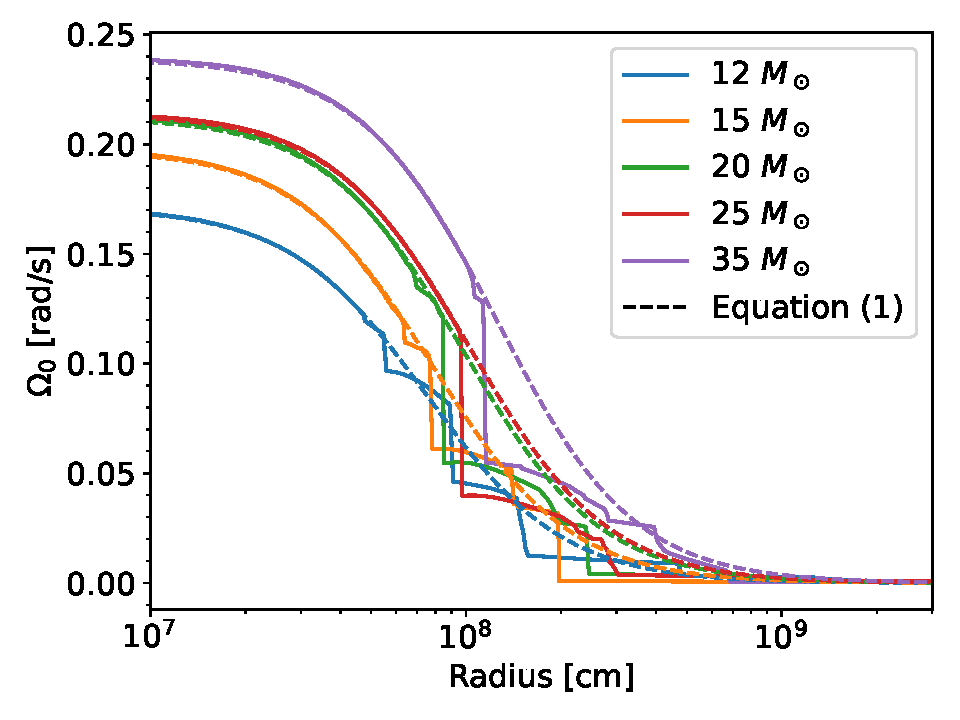
\includegraphics[scale=0.45]{figures/omega_vs_r.pdf}
    \caption{The rotation profiles for five of the \citet{heger:2005} progenitors.  Each solid line represents \citeauthor{heger:2005}'s (\citeyear{heger:2005}) model and the dashed lines are Equation (\ref{eq:omega}) applied to the respective progenitor, with the appropriate differential rotation parameter.  }
    \label{fig:ovsr}
\end{figure}

The core compactness as introduced by \citet{oconnor:2011} is defined as,
\begin{equation}
    \xi_M = \left.\frac{M/M_{\odot}}{R(M_\mathrm{bary}=M)/1000 \text{km}}\right\vert_\mathrm{collapse} ,
\end{equation} 
where we choose $M = 2.5 M_\odot$, and $R(M_{\mathrm{bary}}=M) $ as the radius at which the internal baryonic mass is $2.5M_\odot$, at collapse.  
Figure \ref{fig:a_vs_comp} shows the compactness parameters from the \citet{heger:2005} models (blue stars) plotted against their best fit $A$ values.
A clear linear relation exists between $A$ and $\xi_{2.5}$.  

\begin{figure}[t]
    \centering
    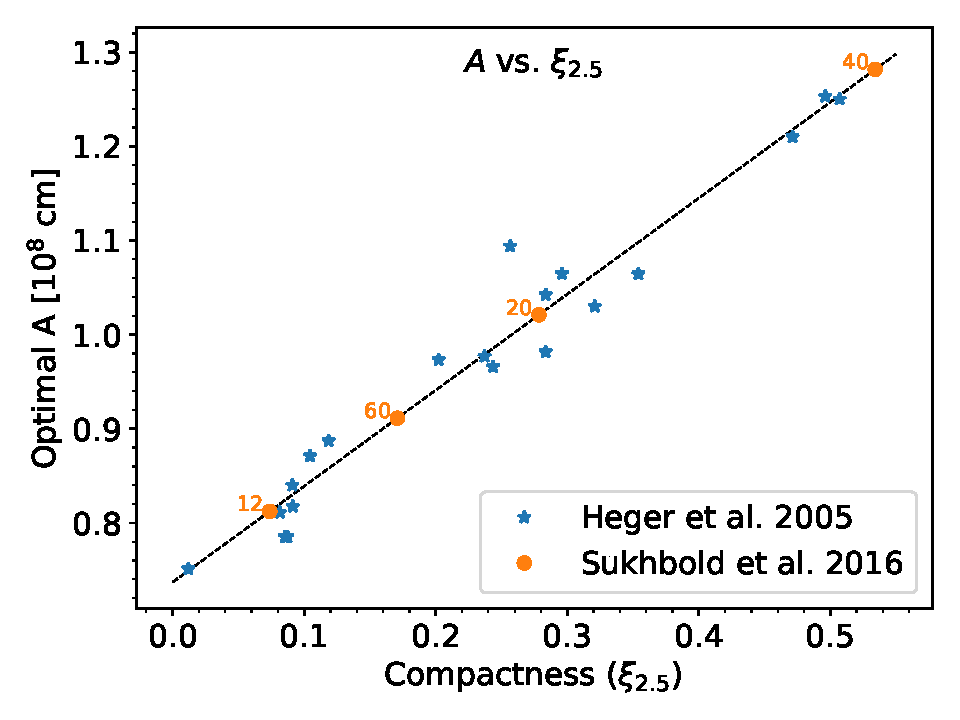
\includegraphics[scale=0.45]{figures/a_vs_compact.pdf}
    \caption{Linear relation between differential rotation parameter, $A$, and compactness parameter of the inner 2.5 $M_\odot$, $\xi_{2.5}$.  The linear trend is constructed from the \citet{heger:2005} rotation profiles.  We then apply the relation to the compactness values from \citet{Suk:2016} to yield the differential rotation parameters.  The progenitor ZAMS masses are labeled in units of $M_\odot$ for each respective point.}
    \label{fig:a_vs_comp}
\end{figure}

\begin{table}[h]
\begin{tabular}{c|c|c}
Progenitor Mass [$M_\odot$] & Compactness & \textit{A}[1000 km] \\
\hline
12  & 0.0738 &         0.8123             \\
20  & 0.2785 &         1.021            \\
40  & 0.5341 &         1.282           \\
60  & 0.1708 &         0.9112          
\end{tabular}
\caption{Listed values for ZAMS mass, compactness calculated from \citet{Suk:2016}, and differential rotation parameter \textit{A}.}
\label{table:compact}
\end{table}

Using this relationship, we calculate optimal $A$ values for the four \citet{Suk:2016} progenitors we use in this work (orange circles in Figure \ref{fig:a_vs_comp}).  
The full list of progenitor masses, compactness values, and A's we use is given in Table ~\ref{table:compact}.  
As a note, we choose to omit the 40 $M_\odot$ progenitor at $\Omega_0 = 3$ rad s$^{-1}$ from our following analysis with a physically motivated rationale.  The $\xi_{2.5}$ value of this progenitor is nearly double that of the 20 $M_\odot$ progenitor (the next closest compactness value).  This fact displays that the 40 $M_\odot$ has a much larger differential rotation parameter compared to the other progenitors, resulting in a nearly-solid body rotation of the core. This endows the core in the 40 \Msun model with drastically more angular momentum than the other models.  The vast amount of angular momentum ultimately led to numerical instabilities in our calculations; thus, we omit the 40 $M_\odot$, with $\Omega_0 = 3$ rad s$^{-1}$ from our analysis.  \\
%So much so, in fact, core bounce is significantly delayed and occurs at much lower central densities due to the strong centrifugal barrier.
%We outline in greater detail the resulting distortion of the GW signal in Section \ref{sec:results}.  Thus, in order to preserve a maximum upper limit on the angular momentum (within a 1.75 $M_\odot$ mass radius) of $\sim 2.4\times 10^{49}$ erg s, we omit the 40 $M_\odot$, with $\Omega_0 = 3$ rad s$^{-1}$ from our analysis.  \\

%V_aniso
%Solberg Hoiland Instability

% 1) 12,15,20,25,35 fit XXX profiles to toy model
% 2) plot optimal A values to compactness from XXX
% 3) plot linear relationship
% 3) Extrapolate to higher masses (w/ given compactness) from XXX


%
%______________________________________________________________


\section{Results}
\label{sec:results}

To extract the GW signal from our simulations, we adopt the dominant, quadrupole moment formula for the gravitational strain, through the slow motion, weak field formalism %\citep[eg.][]{misner:1973,murphy:2009}, 
\citep[eg.][]{finn:1990,blanchet:1990}
\begin{equation}
    h_+ \approx \frac{2G}{Dc^4}
    \frac{d^2I_{zz}}{dt^2},
\label{eq:quad}
\end{equation}
where $I_{zz}$ is the reduced mass quadrupole moment, $G$ is the gravitational constant, $c$ is the speed of light, $D$ is the distance to the source (our fiducial value is $D=10$ kpc), and we assume optimal detector orientation.\\
\par When plotting the amplitude spectral density (ASD) of the GW signal we compute the discrete fourier transform (DFT) consistent with \citet{anderson:2004} and LIGO's implementation,
\begin{equation}
\widetilde{h}_{+k} = \sum^{N-1}_{j=0} h_{+j} e^{-i2\pi jk/N}
\label{eq:dft}
\end{equation}
where $i=\sqrt{-1}$.

To quantify the strength of convection within our simulations, we characterize the anisotropic velocity of the fluid motion within the post shock region according to \citet{takiwaki:2012}:

\begin{equation}
    v_{\mathrm{aniso}} = \sqrt{\left<\rho\Big((v_r - \left<v_r\right>)^2 + v_\theta^2 + v_\phi^2\Big) \right>/\left<\rho\right>}
\label{eq:vaniso}
\end{equation}
where $\left<\right>$ represents an angle average, $v_r$ is the radial velocity, $v_\theta$ is the velocity component in the polar direction, $v_\phi$ is the velocity component in the azimuthal direction, and $\rho$ is the density.  

With the introduction of rotation, a positive angular momentum gradient can be established, leading to inhibited convection, according to the Solberg-H{\o}iland stability criterion.  To quantify this criterion we calculate the condition at the equator for stability in the vertical direction, $R_{\mathrm{SH}}$, consistent with \citet{heger:2000}:

\begin{equation}
    R_{\mathrm{SH}} := \frac{g}{\rho}\Bigg[\Bigg(\frac{d\rho}{dr}\Bigg)_{\mathrm{ad}}-\frac{d\rho}{dr}\Bigg] + \frac{1}{r^3}\frac{d}{dr}(r\omega^2)^2 \geq 0
\label{eq:SHI}
\end{equation}
where $g$ is the local gravitational acceleration, $\rho$ is the density, $(d\rho/dr)_{\mathrm{ad}}$ is the radial density gradient at constant entropy and composition, $r$ is the distance from the axis of rotation, and $\omega$ is the rotational velocity. 

To examine the shape of the shock front, $R_S(\theta,\phi)$, we represent it as a linear combination of spherical harmonics, $Y_l^m(\theta,\phi)$:

\begin{equation}
    R_S(\theta,\phi) = \sum_{l=0}^\infty \sum_{m=-l}^{l} a_l^m Y_l^m(\theta,\phi)
\end{equation}
\begin{equation}
    Y_l^m = \sqrt{\frac{2l+1}{4\pi}\frac{(l-m)!}{(l+m)!}}P_l^m(\cos(\theta)) e^{im\phi}
\end{equation}
where $P_l^m$ are the associated Legendre polynomials \citep{burrows:2012,takiwaki:2012}.  However, because of the two dimensional nature of our simulations $\phi = 0$ and all $m = 0$ as well; thus the coefficients $a_l^0$ are

\begin{equation}
    a_l^0 = \int_0^\pi d\theta \sin(\theta)R_S(\theta)Y_l^0(\theta) .
\label{eq:sho_coeff}
\end{equation}
It follows that $a_0^0$ corresponds to the average shock radius.
\subsection{Rotation's Influence on Shock Front Evolution}

\begin{figure}[t]
    \centering
    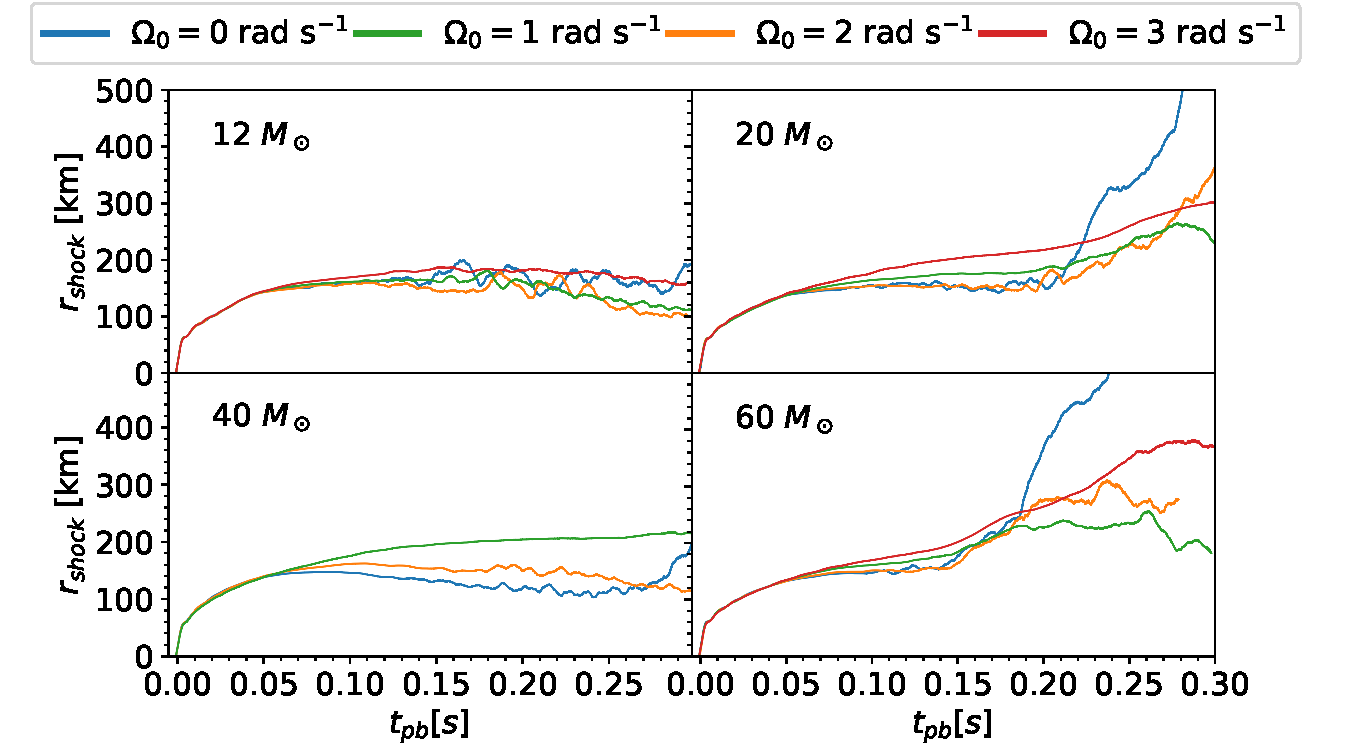
\includegraphics[width = 0.5\textwidth]{figures/M1_shock_mass_raster.pdf}
    \caption{Shock radius evolution of the four progenitor models versus time (post bounce).  As different progenitors evolve at different rates, they may not have enough time to revive their shock front within the 300 ms interim.  As such, only the nonrotating 20 \Msun and 60 \Msun progenitors show substantial shock expansion. }
    \label{fig:shock}
\end{figure} 

While our focus in the present work is on the GW signals up to 300 ms post bounce, we briefly discuss the impact of rotation on the evolution of the shock front as it propagates outward.  In certain cases, independent of the mechanism, the shock front may require over 300 ms to revive and complete a successful explosion.  Because our simulations are only run until 300 ms pb, we refrain from asserting which progenitors successfully explode.  Rather, we remark on how the average shock radii develop with time.

Of our 15 simulations, only the nonrotating 20 \Msun and 60 \Msun progenitors show substantial shock expansoin.  The effect rotation has on reviving the shock is not a simple one. 
In one respect, one expects greater centrifugal support to lead to a larger shock front.  However, there are two factors that inhibit the shock from propagating outward.  The first is the inhibited convection due to the positive angular momentum gradient within the progenitor. Weaker convection results in less efficient neutrino heating \citep{dolence:2013, murphy:2013} and less positive support from turbulence in the gain region \citep{couch:2015a, mabanta:2018}.  The  second rotational element that inhibits explosions is the lack of neutrino production.  Rotation centrifugally supports matter that is infalling during the initial collapse of a star.  As such, the collapsing material does not settle as deeply into the gravitational potential of the stellar core, thereby creating an explosion that has less energy.  This process results in a lower neutrino luminosity and slower contraction of the PNS \citep{summa:2018}. 
These two dominant effects, weaker convection and reduced neutrino luminosity, can create an unfavorable scenario for a supernova explosion that is revived by neutrino heating.

This is not universally true, however. 
Some of our rotating models ($\Omega_0 = 3$ rad s$^{-1}$, 20 \Msun \& 60 \Msun) have advancing shock radii.  With longer simulation times, these could lead to explosion.  In these cases, it seems that rotation could be sufficiently rapid to overcome the deleterious effects on convection and reduced neutrino luminosity.
Similar non-monotonic behavior is reported by \citet{summa:2018} in their 2D simulations.
Hence, the introduction of rotation involves competing forces that can enhance or diminish the shock.  Figure \ref{fig:shock} shows the average shock radius evolution versus time (post bounce) over our entire parameter space.

%In the case of the 12 \Msun progenitor, the mean shock front reaches 400 km and continues to expand around 400 ms post bounce.  For its rotating cases, the shock front reaches its peak value at 150 ms post bounce and recedes to 100 km for the remainder of the simulations, most likely due to the inhibited convection in the gain region.  The 20 \Msun similarly explodes for the nonrotating case.  However, $\Omega_0 = 1$ shows a peak at 270 ms post bounce and receding thereafter.  Both higher rotational velocities exhibit more energetic behavior as their shock front propagates outward, with the $\Omega_0 = 3$ case successfully passing 400 km and continuing to become less bound.  Sufficient entropy in the gain region powers the explosion of the 40 \Msun progenitor.  For the $\Omega_0 = 2$ case, the shock front becomes more active nearly 200 ms later, expanding at a rate of 1000 km/sec.  The 60 \Msun progenitor likewise explodes in the nonrotating case.  While the $\Omega_0 = 3$ simulation exceeds 400 km, it stalls soon after and begins recede deeper into the gravitational potential.  

%What remains physically consistent, however, is that rotation delays runaway shock expansion across all progenitor masses.

\subsection{Comparison to CFC GR}

 \begin{figure}[t]
    \centering
    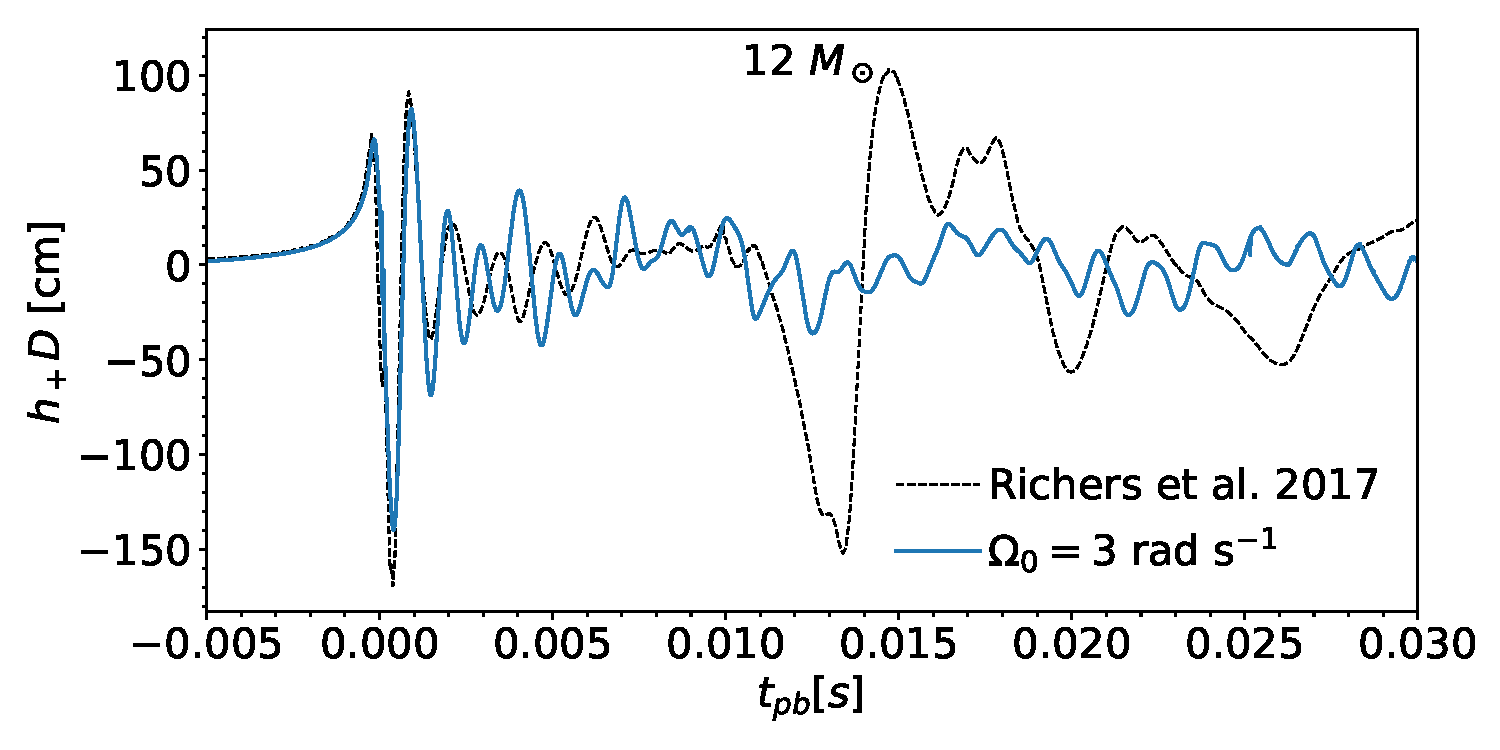
\includegraphics[width=0.48\textwidth]{figures/bounce_richers.pdf}
    \caption{GW strain vs. time (post bounce) for a 12 \(M_\odot\) progenitor with $\Omega_0 = 3$ rad s$^{-1}$.  Plotted in the dashed line is the GW strain from \citet{richers:2017} using the CFC \texttt{CoCoNuT} code and the solid line is our result using the relativistic effective potential coupled with Newtonian dynamics.  While the different grids and treatment of hydrodynamics lead to differences in the strain in the early post bounce phase, we qualitatively verify our gravitational treatment by obtaining a nearly exact bounce signal. }
    \label{fig:bounce_cfc}
\end{figure}

\begin{figure*}[t]
  \centering     %%% not \center
  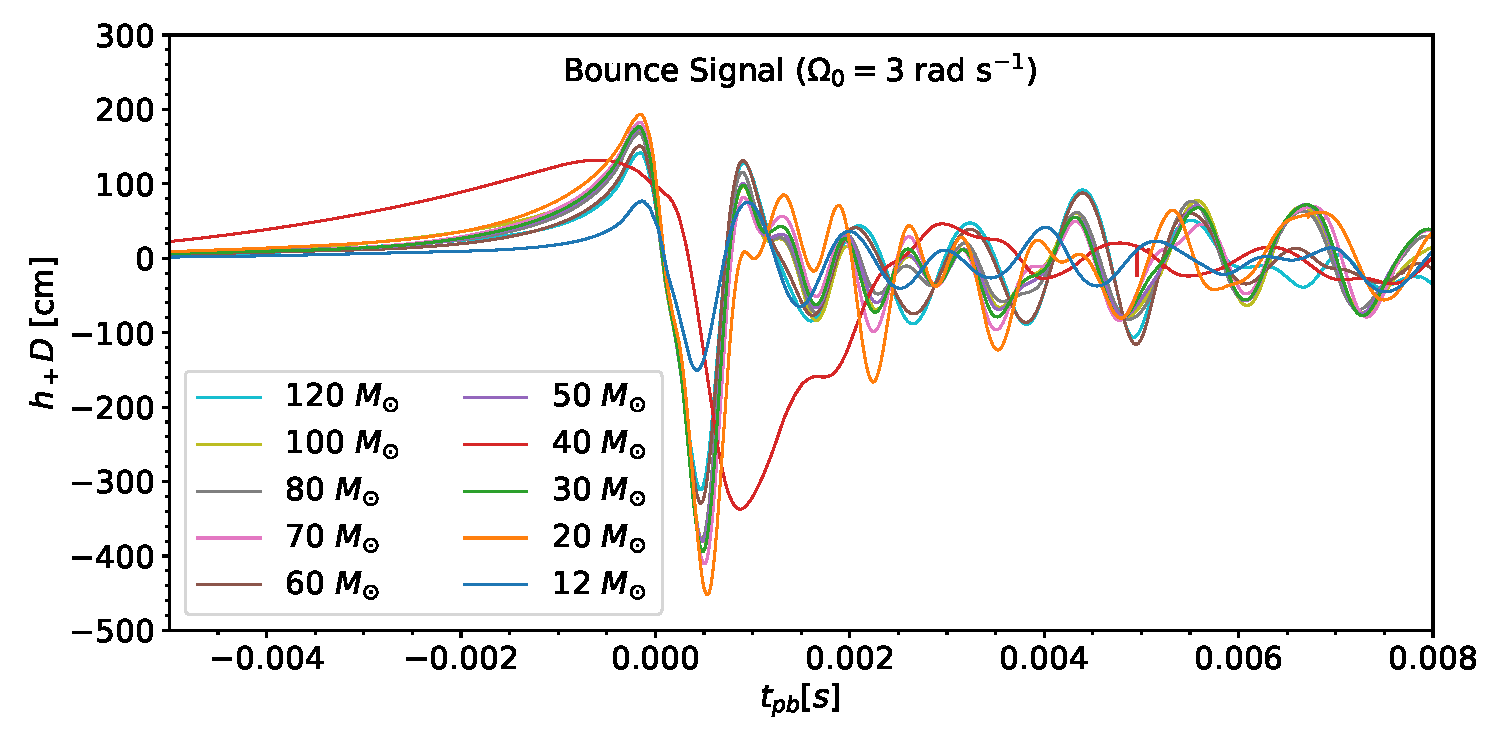
\includegraphics[width=0.49\textwidth]{figures/hd3_bounce_test.pdf}
  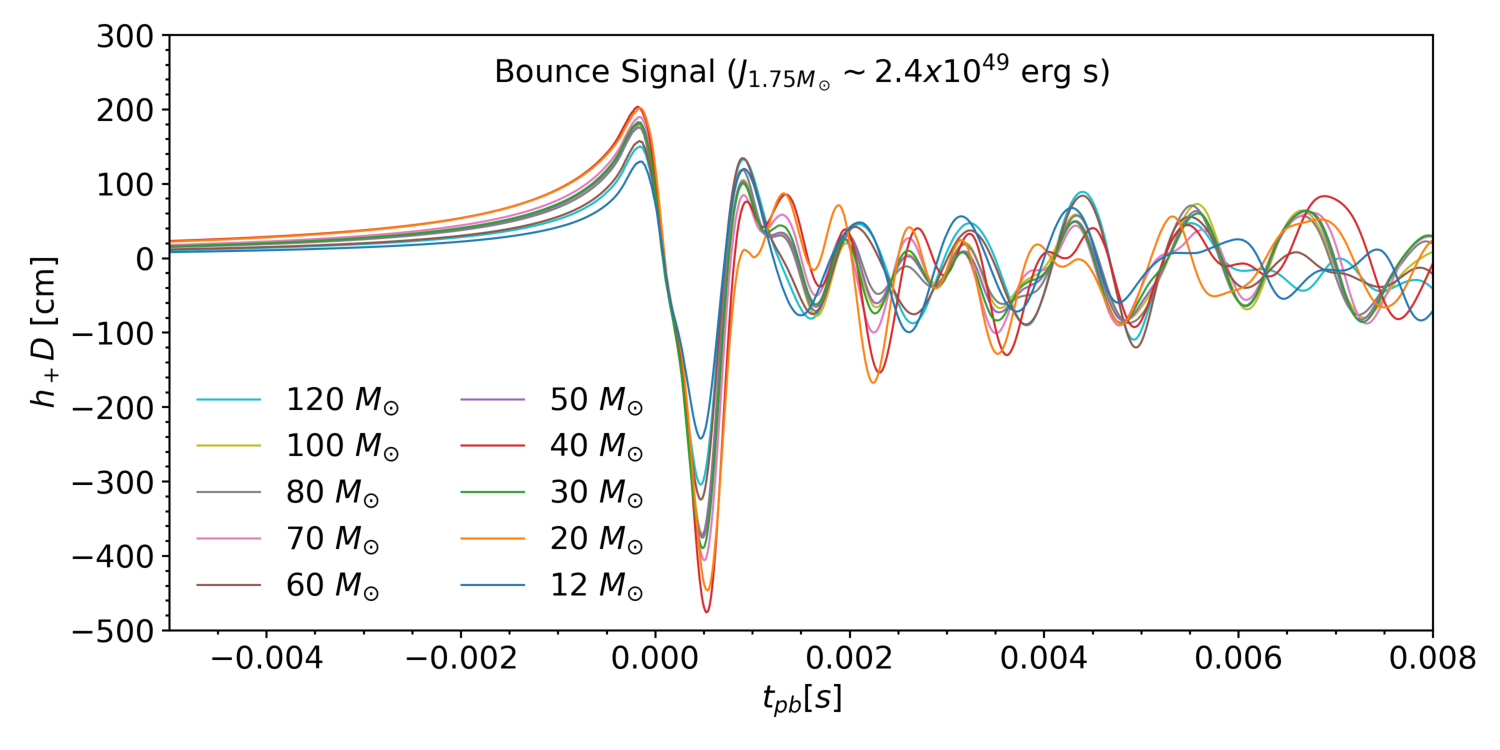
\includegraphics[width=0.49\textwidth]{figures/hdj_bounce_final.pdf}
  \caption{(Left) GW bounce signal from all 10 progenitor masses with $\Omega_0 = 3 \text{ rad s}^{-1}$.  By applying Equation (\ref{eq:omega}), we assign a radially dependent, angular velocity to our progenitors.  Because the central density profiles of each progenitor are different---namely a less compact $12\,M_\odot$ and more compact $40\,M_\odot$---the progenitor cores are endowed with different amounts of angular momenta.   (Right) Modified bounce signals after adjusting rotation rates to yield similar angular momenta ($\sim 2.4\times10^{49} \text{erg s}$) of the inner $1.75\,M_\odot$ of matter.  As predicted by \citet{dimm:2008} and \citet{abdik:2010,abdik:2014}, the GW bounce signals depend on the inner core angular momentum at bounce, not the original ZAMS mass.}
  \label{fig:bounce}
\end{figure*}

In multidimensional simulations of CCSNe, the treatment of gravity must offer a balance between numerical accuracy and computational cost.   The CFC offers a nearly identical GW signal, compared to full general relativity (GR), while reducing simulation time \citep{ott:2007}.  Figure \ref{fig:bounce_cfc} offers a qualitative check of our effective general relativistic potential compared to CFC \citep{richers:2017}.  We incorporate an identical deleptonization profile \citep{lieb:2005} and SFHo EOS \citep{steiner:2013}.  Moreover, we match the differential rotation parameter and rotation profile by selecting an $A = 634$ km and $\Omega_0 = 3$ rad s$^{-1}$.  For this comparison, we match the neutrino physics of their simulation by using a ray-by-ray, three species, neutrino leakage scheme \citep{oconnor:2010,couch:2014}.  We capture a nearly identical bounce signal and similar strain up to 5 ms post bounce. \par
However, after the initial bounce signal ring-down, it is clear that the different computational treatments of hydrodynamics and grid geometry result in differences in the GW strains.  Although not exact, the efficiency of the effective general relativistic potential offers a reasonable method to accurately model the GW signal from CCSNe to within 10\% and allows for larger sweeps of parameter space \citep{muller:2013}.

%-----------------------------------
%-----------------------



\subsection{ZAMS Influence on Gravitational Bounce Signal}

%%begin comment
\iffalse

%entropy slice
\begin{figure*}[t!]
  \centering     %%% not \center
  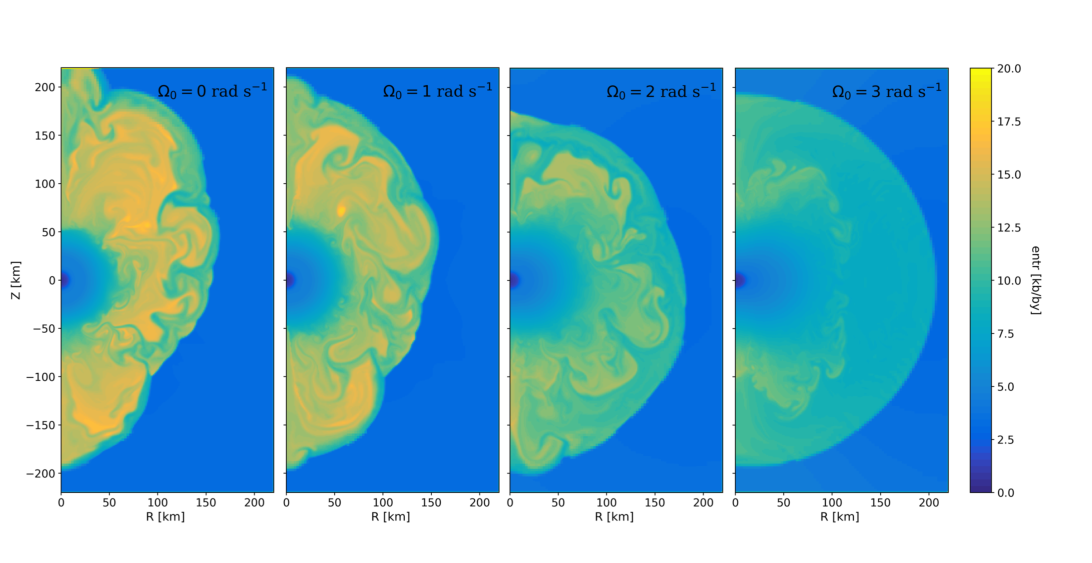
\includegraphics[width=\textwidth]{figures/entr_slice_2.pdf}
  \caption{Entropy slices for the 60 \Msun progenitor at 150 ms post bounce.  The increased rotational velocity centrifugally restricts SASI activity in the polar direction, thereby inhibiting excitation of the g modes of the PNS.  Moreover, the positive angular momentum gradient inhibits convection and neutrino heating, reflected in the lower entropies in the post shock region.}
  \label{fig:entr_slice}
\end{figure*}
\fi
%%end comment

While different progenitors $\gtrsim$$8\, M_\odot$ will experience widely varied evolution, once their iron cores reach the effective Chandrasekhar mass \citep{baron:1990} and collapse commences, the physics of the of collapse becomes somewhat universal.
In particular, the mass of the homologously collapsing inner core is fixed more by microphysics than by the macrophysics of varied stellar evolution. 
This nearly identical inner core mass across ZAMS parameter space yields similar core angular momenta, for identical rotation rates.  Hence, the core bounce signal is nearly indistinguishable between progenitor masses.  For further verification of our gravitational treatment, we perform 12 additional simulations using neutrino leakage---from collapse---until eight milliseconds after core bounce, in order to replicate this bounce signal degeneracy, using the \citet{Suk:2016} progenitors.  Outlined by \citet{ott:2012}, neutrino leakage has a small effect on the GW bounce and early post bounce signal.  
Moreover, our results are consistent with 3D, fully general relativistic predictions given by \citet{ott:2012}, that similar core angular momenta yield similar GW bounce signals.  

Figure \ref{fig:bounce} displays the bounce signals for all 10 progenitor masses, ranging from 12 \Msun -- 120 \Msun.  The left panel is for uniform rotational velocity prescriptions at $\Omega_0 = 3\text{ rad s}^{-1}$.  As previously highlighted, the angular momentum of the inner core is the main contributor to the gravitational bounce signal.  While many of the waveforms have similar amplitudes, there are two clear outliers: the $12\,M_\odot$ and $40\,M_\odot$ progenitors.  The $12\,M_\odot$ and $40\,M_\odot$ progenitors respectively have lower and higher compactness values at collapse, by nearly a factor of two.  Because we endow each progenitor with angular velocity, and not specific angular momentum, the more compact $40\,M_\odot$ progenitor will receive more angular momentum, compared to the remaining progenitors, thereby affecting the resulting GW bounce signal.  As outlined by \citet{dimm:2008}, once a star is sufficiently rotating, the centrifugal support slows the bounce, diminishing the GW bounce amplitude and widening out the bounce peak of the waveform.  

The inverse is true for the $12\,M_\odot$ case.  Because it has a less compact, inner core at collapse, use of Equation (\ref{eq:omega}) leads to less initial angular momentum, thereby producing a lower amplitude bounce signal.  After modifying the initial rotation rates of both progenitors, to match the progenitor core angular momenta (right panel of Figure \ref{fig:bounce}), the change produces nearly identical GW bounce signals.  

Hence, our results from exploring the bounce signal over a wide range of progenitor masses support the results of previous studies of angular momentum dependence of the GW signal \citep{dimm:2008,abdik:2010,abdik:2014}, but also serve as a cautionary note for future groups who perform rotating CCSN simulations with a wide variety of progenitor models.  
It is worth noting that other rotational treatments exist beyond the simple angular velocity law, such as specifying a radial, specific angular momentum profile \citep[eg.][]{oconnor:2011}, or using the rotational profile from the rotating stellar evolution models directly \citep{summa:2018}.

\subsection{Rotational Influence on Accretion Phase Gravitational Wave Emission}

Our results in the previous section support the efficacy of our effective GR potential for accurately modeling the GW signals from CCSNe.
We now turn to exploring the rotational effects on the GW signal during the accretion phase, up to 300 ms after bounce.


While the consistency of the inner core mass for collapsing iron cores creates a setting where envelope mass has little effect on the bounce signal, the post bounce dynamics of the explosion largely depend on the mass surrounding the PNS.  For nonrotating CCSNe, the shock front propagates outward, and loses energy due to dissociation of iron nuclei and neutrino cooling.  In the case of rotation, the initial progenitor and resulting shock front become more oblate.  Rotation can affect the GW emission in three respects: the post shock convection is damped, the SASI becomes restricted, and the PNS vibrational modes are inhibited. 

  As the $\Omega_0$ value increases in our models, a positive angular momentum gradient is established within the post shock region, partially stabilizing it to convection via the Solberg-H{\o}iland instability criterion \citep{endal:1978,fryer:2000}.  We quantify the reduced convection in Figure \ref{fig:vaniso}.  Brighter colors correspond to higher values of the anisotropic velocity as outlined in Equation (\ref{eq:vaniso}).  As expected, the convection in the gain region is reduced with increasing rotational velocity.  To tie this inhibited convection to the Solberg-H{\o}iland instability criterion, we follow the prescription of Section 2.3.2 of \citet{heger:2000}.  We quantify this instability criterion as outlined in Equation (\ref{eq:SHI}) by taking slices along the equator and tracking its evolution.  Figure \ref{fig:SHI} displays the $R_{\mathrm{SH}}$ value along the equator of the 12 \Msun progenitor for all four rotational velocities.  As the $\Omega_0$ increases, the propensity for convection (colored blue) within the post shock region clearly decreases.  This inhibited convection results in weakened turbulent mass motion within the gain region, thereby reducing the GW amplitude at later times.  %Figure \ref{fig:ccsn_all} clearly displays the trend of decreasing GW amplitude with increasing rotational velocity, over all progenitor masses, and displays that   the muting of late time GWs in our 2D simulations manifests itself as a universal trend.
 
%In Figure \ref{fig:entr_slice} we show a progression of entropy slices  for the 60-\Msun progenitor at 150 ms pb, for all values of $\Omega_0$.  As rotation becomes stronger, the entropy in the gain region decreases, reflecting the weakened convective activity.  
Furthermore, we recast our analysis by focusing on regions within the CCSN that emit GWs.  The lower panel of Figure \ref{fig:region} displays the inhibited convective signal with increasing rotation, as the GW signal in the gain region becomes increasingly muted.  The typical convective signals in the early post bounce regime are then quickly washed out by the post bounce ring down of the PNS, as rotation increases.

\begin{figure}[]
    \centering
    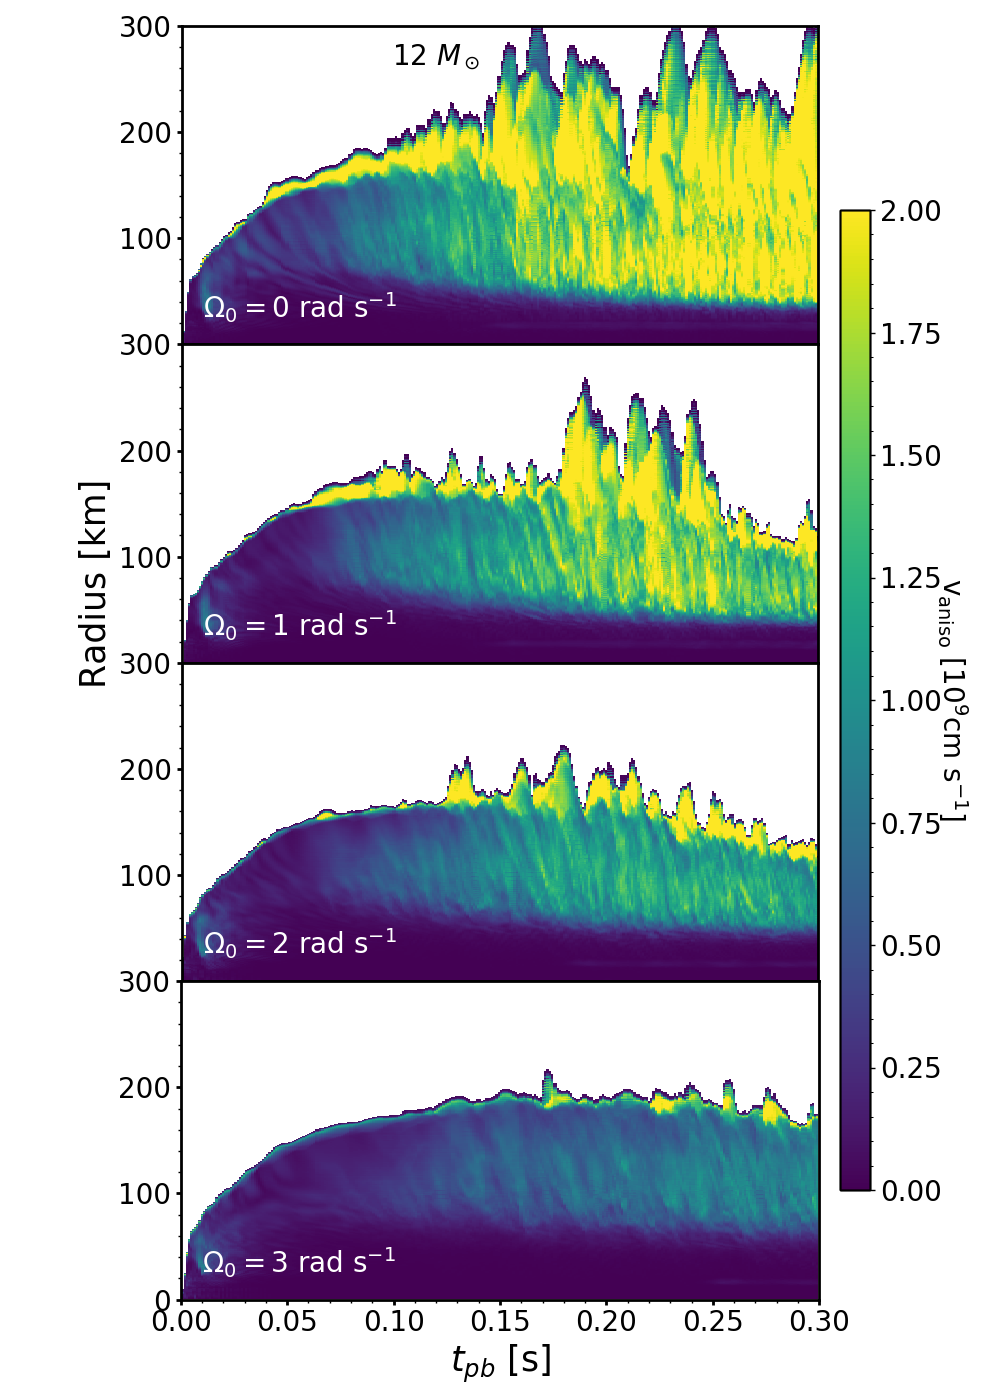
\includegraphics[width=0.5\textwidth]{figures/vaniso_test.png}
    \caption{Spherically averaged anisotropic velocity of the post shock region for the 12 \Msun progenitor.  Brighter colors correspond to increased convection in the post shock region according to Equation (\ref{eq:vaniso}).  As rotational velocity increases, convective activity is inhibited.}
    \label{fig:vaniso}
\end{figure}

\begin{figure}[]
    \centering
    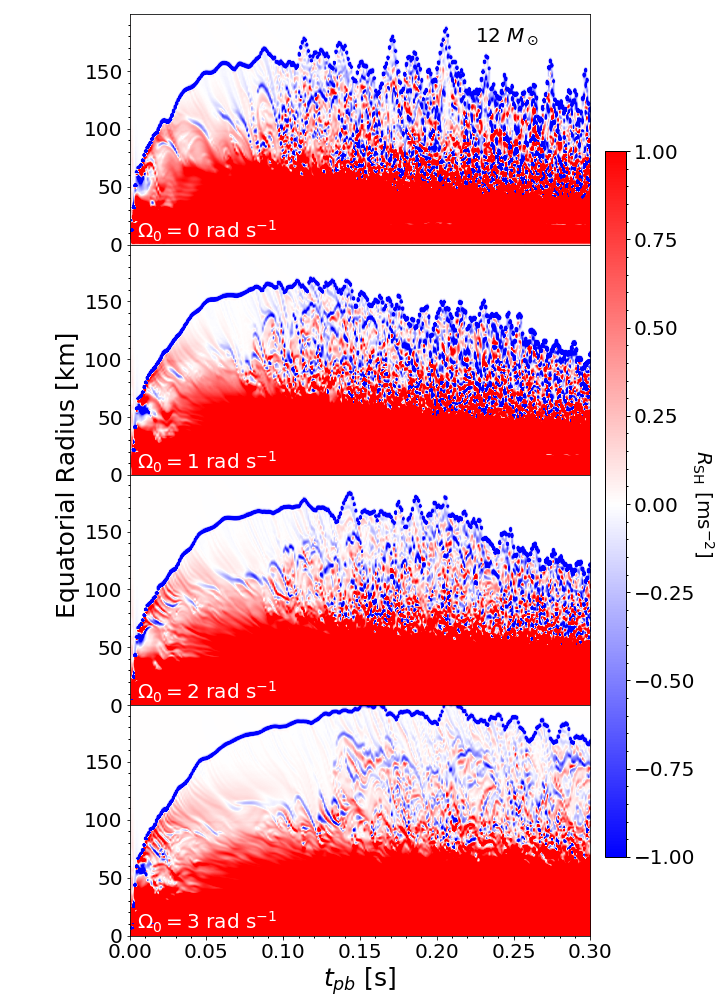
\includegraphics[width=0.5\textwidth]{figures/SHI_test.png}
    \caption{Slices along the equator of the 12 \Msun progenitor at each rotational velocity.  Colors correspond to the Solberg-H{\o}iland stability criterion, $R_{\mathrm{SH}}$, from Equation (\ref{eq:SHI}).  As rotational velocity increases, not only does the convectively stable band in the core grow (seen in red), but the amount of convection within the post shock region (seen in blue) decreases as well.  The differences in shock radius evolution between Figure \ref{fig:vaniso} and the above Figure arise because Figure \ref{fig:vaniso} uses an angular average over the domain, whereas the above Figure uses equatorial slices.}
    \label{fig:SHI}
\end{figure}

 \begin{figure*}[htp]
  \centering     %%% not \center
  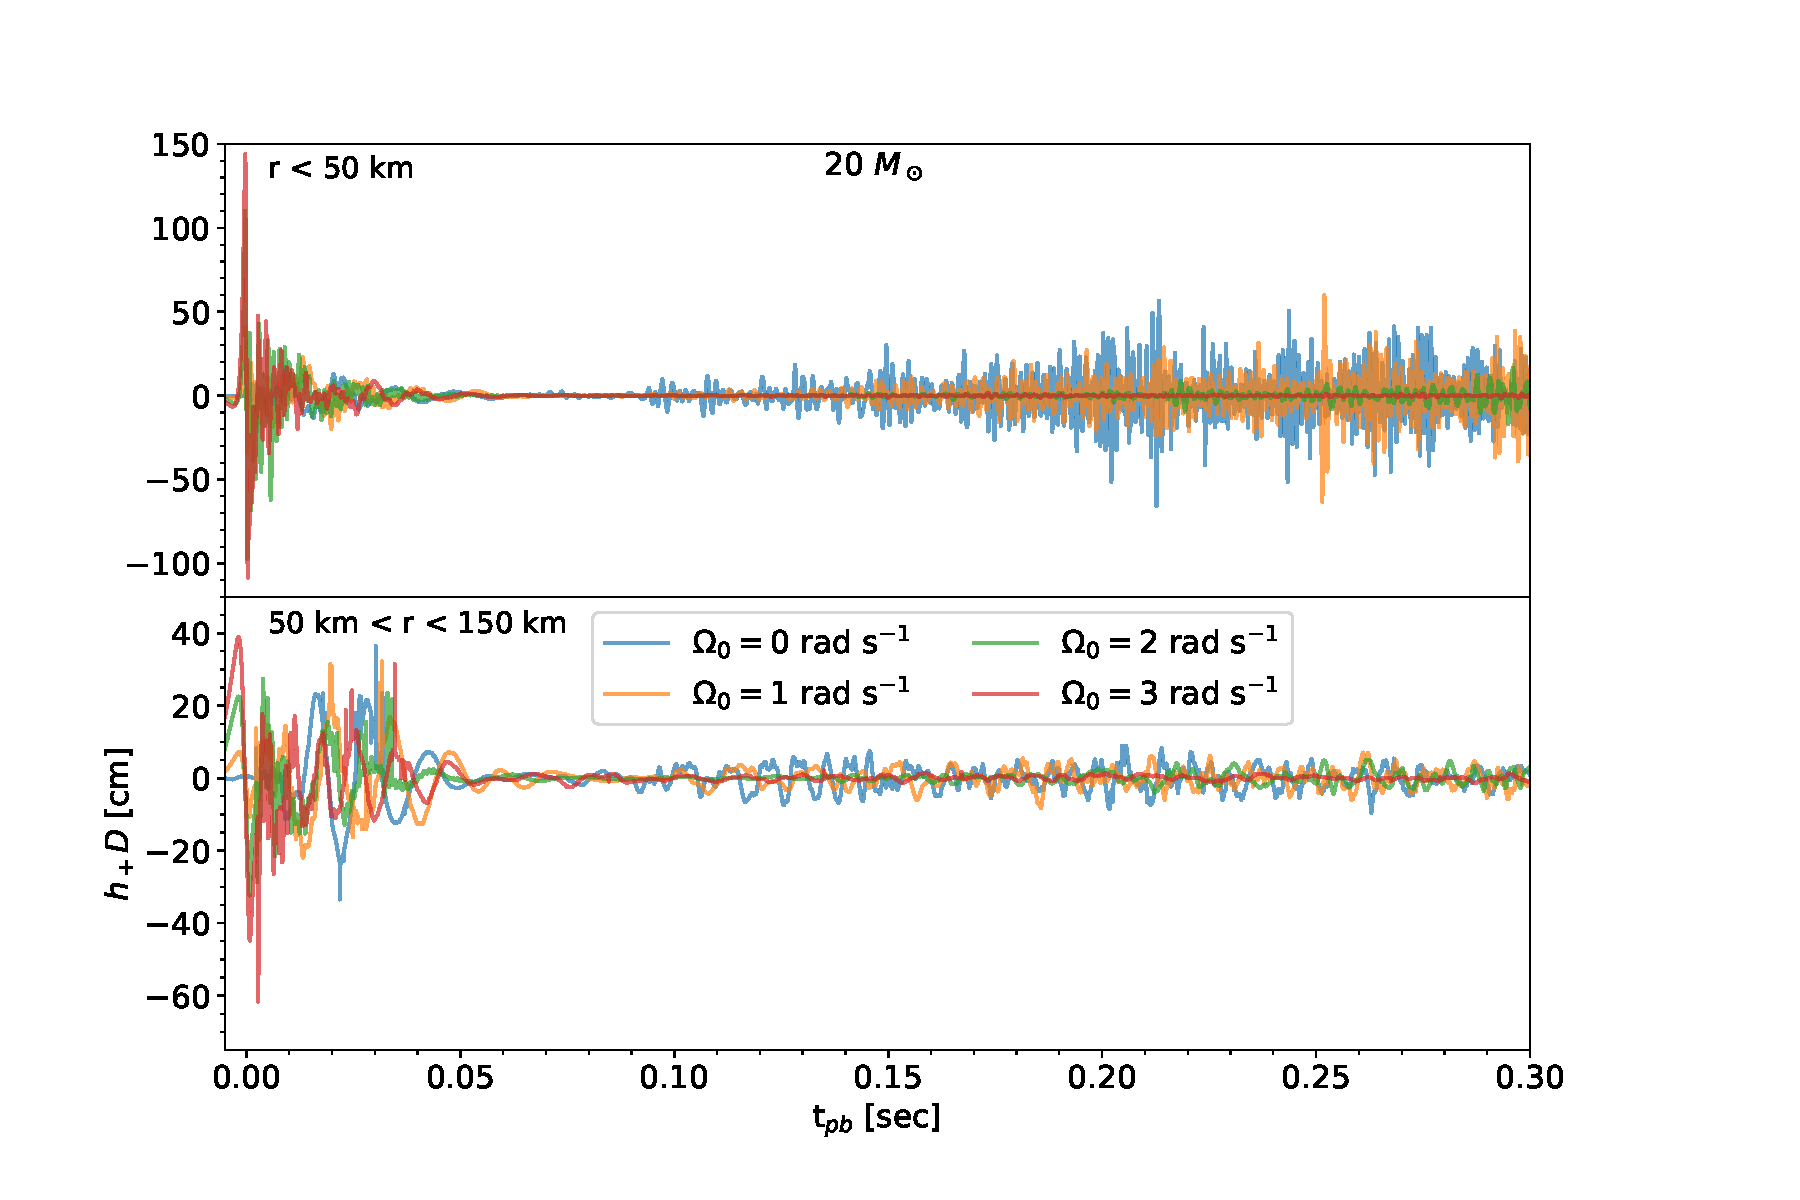
\includegraphics[width=\textwidth]{figures/tdwf_region_20.pdf}
  \caption{Time domain waveforms for the 20 $M_\odot$ progenitor.  Each panel corresponds to the region from which the GWs are emitted.  The large contribution in the top panel indicates the main source of late time GWs is from the vibrating PNS.  The middle panel displays the inhibited convective signal $\sim 50-100 $ ms post bounce that is characteristic of this quiescent phase.}
  \label{fig:region}
\end{figure*}

\begin{figure}
    \centering
    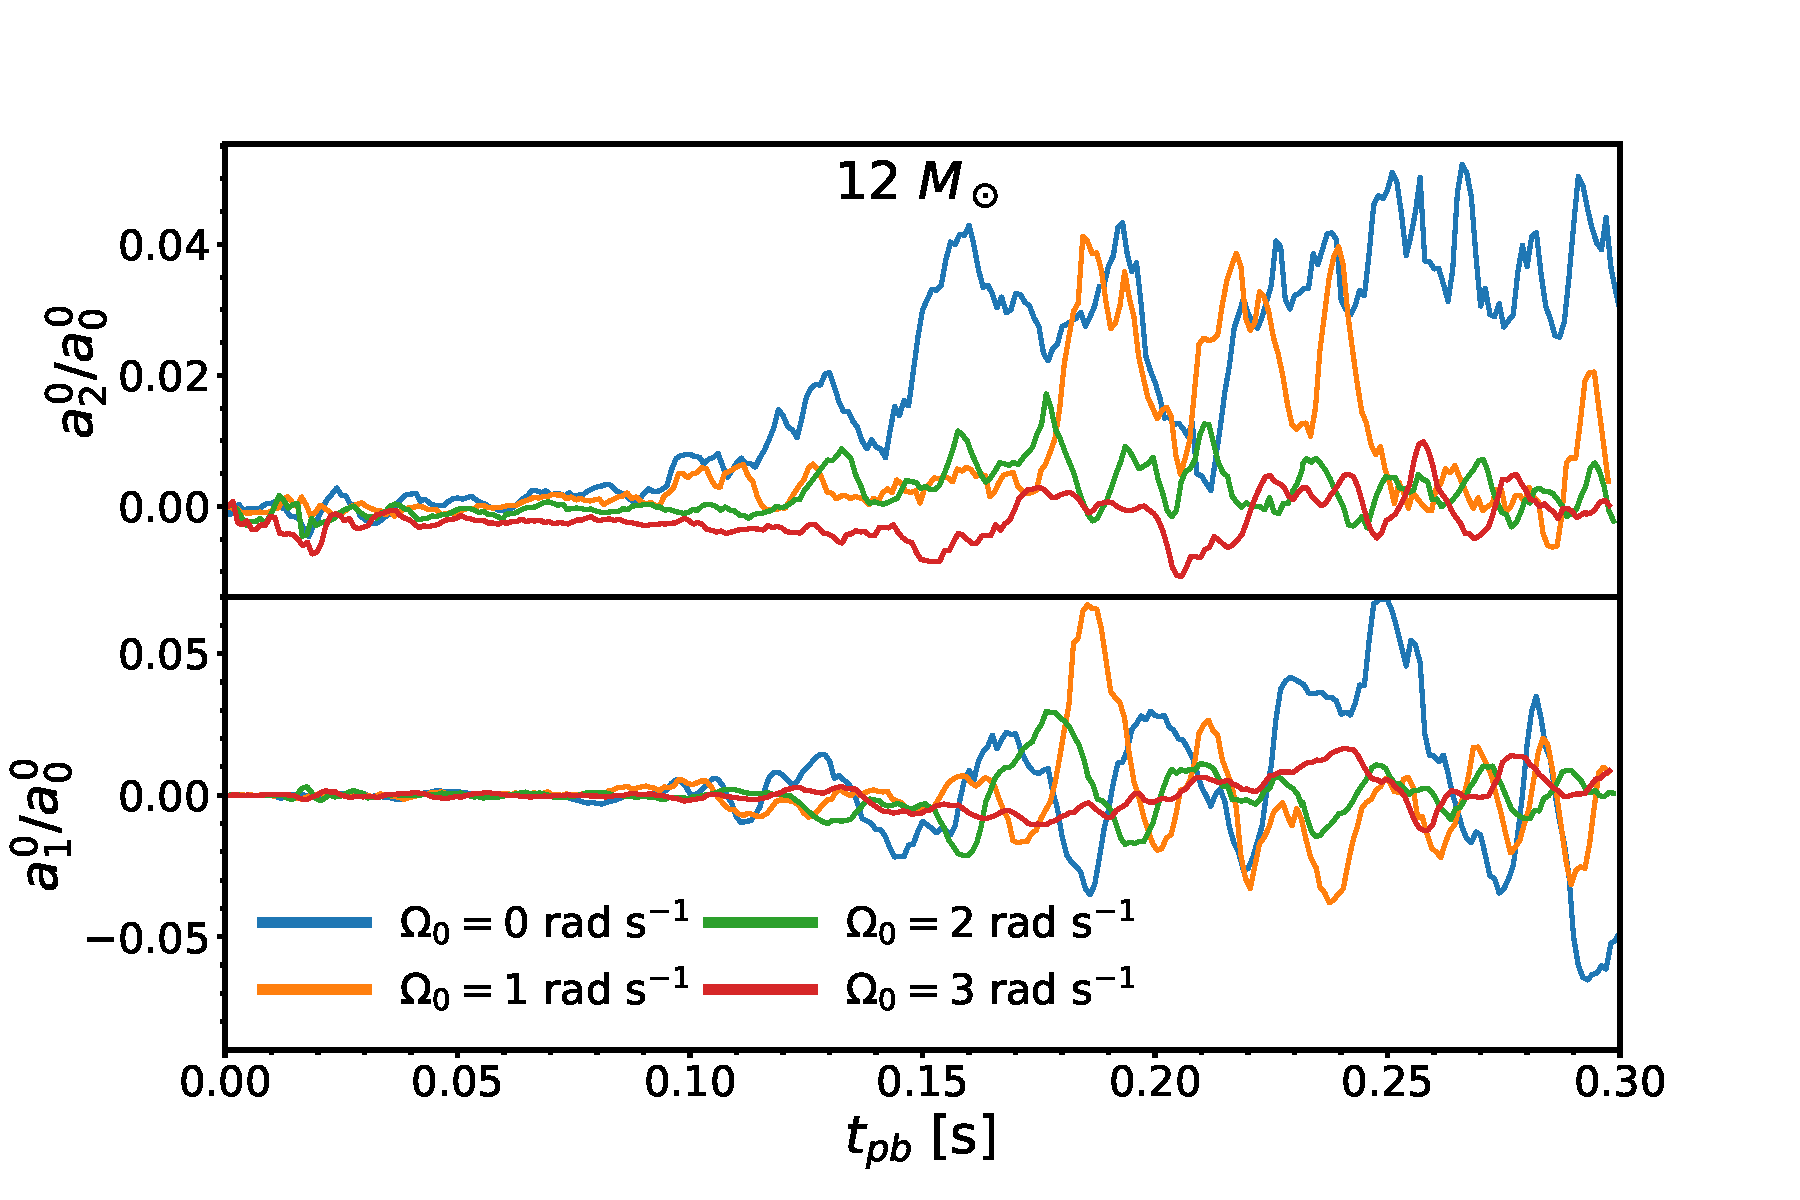
\includegraphics[width=0.5\textwidth]{figures/sasi_axis_norm.pdf}
    \caption{Coefficients from spherical harmonic decomposition of the shock front, outlined in Equation (\ref{eq:sho_coeff}).  The $a_1^0/a_0^0$ and $a_2^0/a_0^0$ terms describe the overall dipole and quadrupole nature of the shock front, respectively.  As the SASI is one of the main contributors to creating asymmetries in the shock front, the lower $a$ values correspond to a more spherical shock, or one with diminished SASI.}
    \label{fig:sasi}
\end{figure}

%4 panel GW strain plot
\begin{figure*}[t]
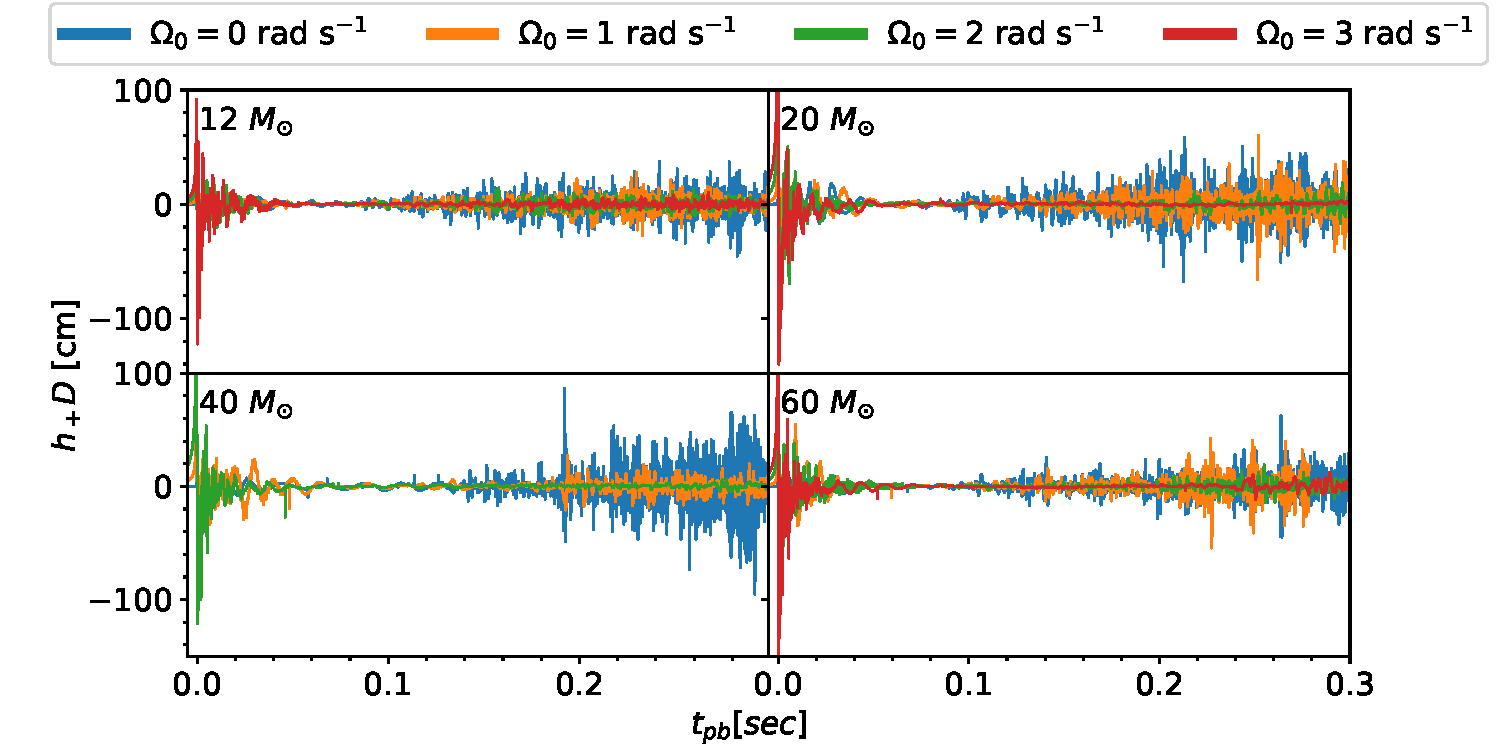
\includegraphics[width=\textwidth]{figures/ccsn2D_M1_all.pdf}
\centering
\caption{Time domain waveforms over our entire parameter space.  For all four progenitor masses, the rotational muting of the GW signal is clear in the late post bounce regime.  While there is some weak dependence in the character of the late-time GW signals with progenitor ZAMS mass, the rotational muting occurs for all progenitors.}
\label{fig:ccsn_all}
\end{figure*}

\begin{figure}[t]
    \centering
    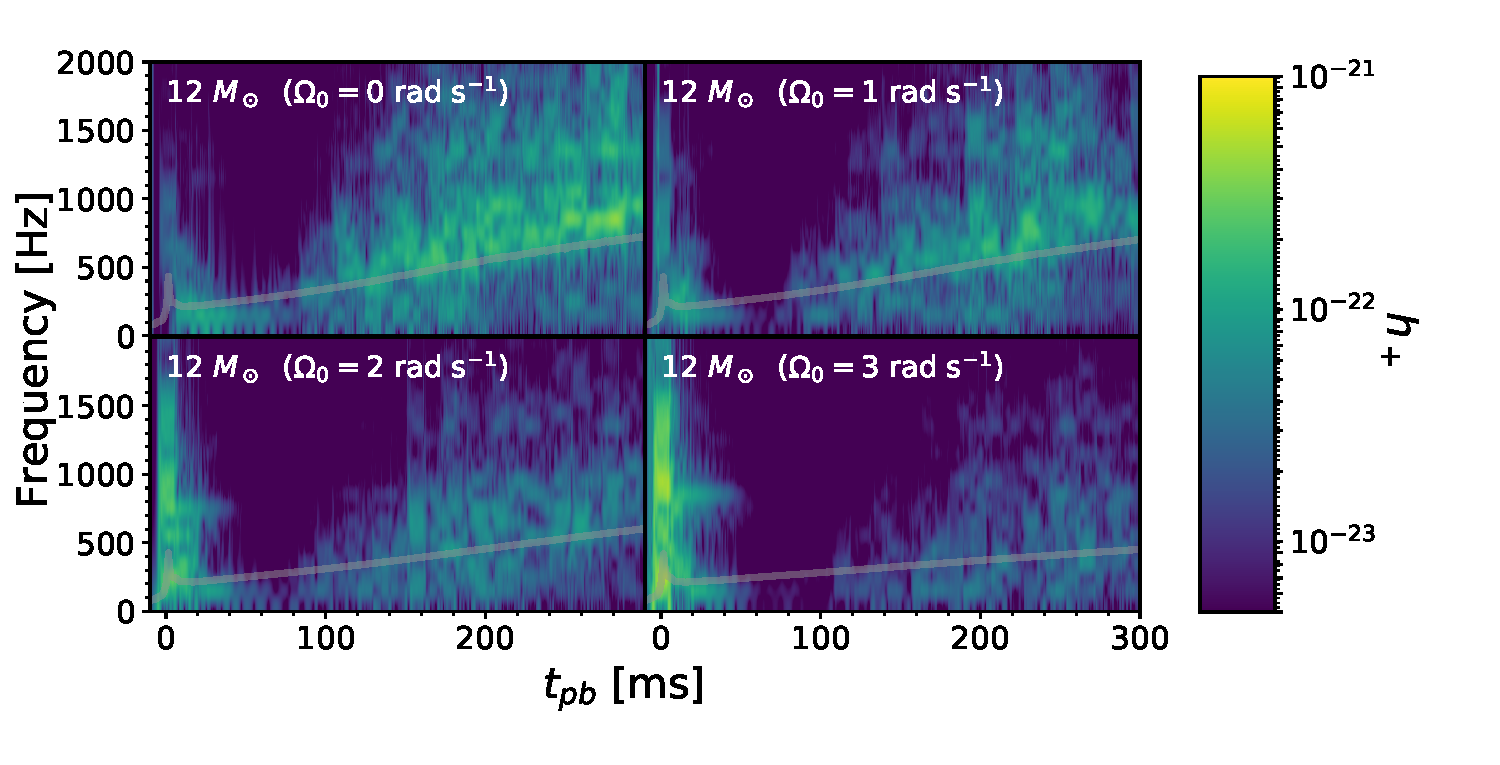
\includegraphics[scale=0.38]{figures/gws_2x2_line_M1.pdf}
    \caption{Spectrograms for the $12 M_\odot$ progenitor over all four rotational velocities.  The key aspects revealed by the spectrogram are the rotational muting of GWs and the flattening of the signal from the surface g-mode of the PNS.  This flattening is a product of the enlarged radius of the PNS due to centrifugal effects and can be characterized by the dynamical frequency ($f_{dyn} = \sqrt{G \overline{\rho}}$), overlaid in grey.}
    \label{fig:2x2}
\end{figure}

\begin{figure*}[t!]
  \centering     %%% not \center
  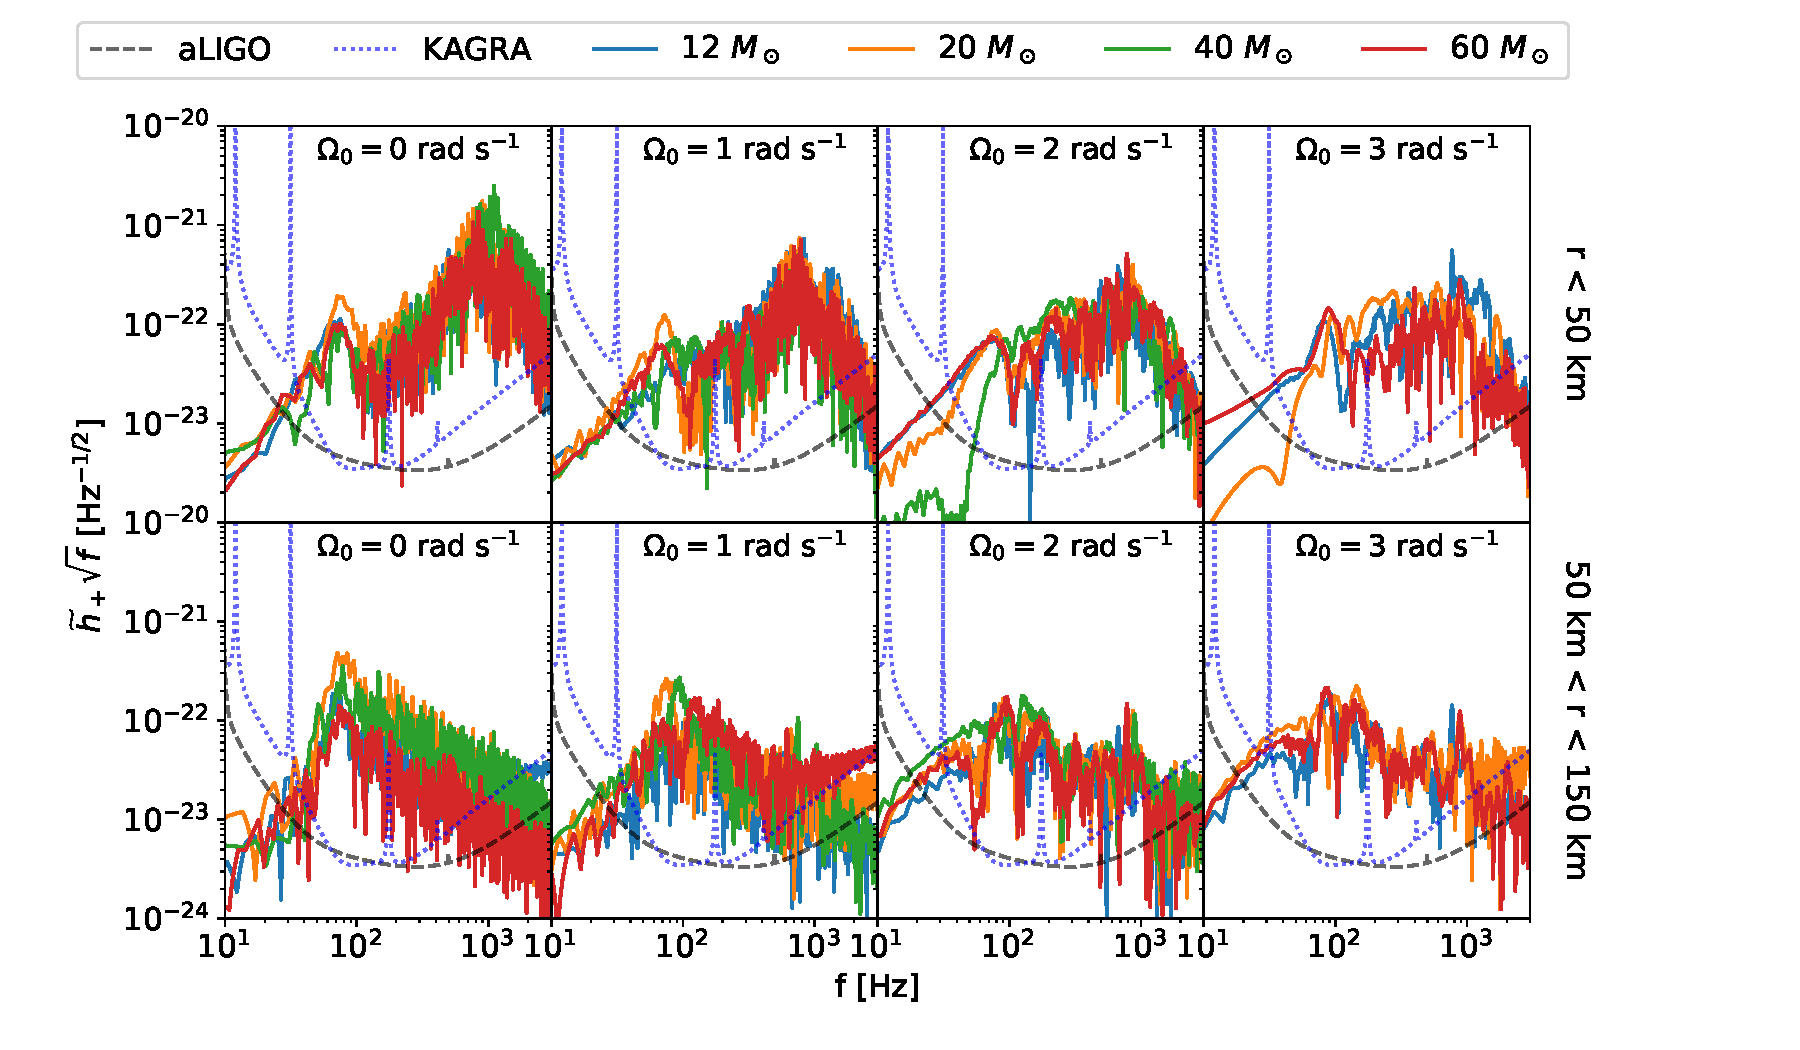
\includegraphics[width=\textwidth]{figures/tbe6tbe300_combined_M1_long.pdf}
  \caption{Amplitude spectral density (ASD) plot of all progenitors for all rotation rates from $t_{be}+6$ ms $\rightarrow t_{be}+300$ ms.  The rotational muting of the fundamental PNS g-mode is displayed as the peak frequency ($\sim 800$ Hz) becomes less prevalent, with increasing rotation rate.  Likewise, the low frequency signals ($\sim30$ Hz) become more audible, with increasing rotational velocity.  Plotted in the black dashed line is the design sensitivity curve for aLIGO in the zero detuning, high sensitivity configuration \citep{barsotti:2018}.  The blue dotted line is the predicted KAGRA detuned, sensitivity curve \citep{komari:2017}.}
  \label{fig:spetra_long}
\end{figure*}

Under typical nonrotating conditions, the shocked accretion flow will grow unstable from the nonradial deformation modes and amplify to eventually become a dominant driver in reviving the shock; this effect is also known as SASI \citep{scheck:2008,marek:2009a}.  In 2D simulations, the SASI excites large, oscillatory flows along both poles that drives changes in entropy, capable of causing post shock convection.  It is worth noting in 3D simulations, the SASI can excite `spiral' modes that correspond to nonzero $m$ values \citep{blondin:2007,kuroda:2016}.  The high degree of nonlinearity between the hydrodynamic flows, neutrino interactions, and gravitational effects can yield matter flow that is quadrupolar, thereby resulting in GW emission.  However, when the shock becomes restricted in the polar direction, due to centrifugal effects, SASI development is inhibited.  To quantify the role of SASI, we decompose the shock front into coefficients based on the spherical harmonics, $Y_l^m$, according to Equation (\ref{eq:sho_coeff}). Figure \ref{fig:sasi} illustrates the evolution of the $a_1^0$ and $a_2^0$ coefficients over time.  Both coefficients quantify the deviation of the shock from spherical symmetry.  Specifically, the $a_1^0$ term describes the overall dipole nature of the shock, and the $a_2^0$ term describes its quadrupole nature.  Both coefficients are normalized by the mean shock radius, $a^0_0$.  Clearly, both approach zero with increasing rotational velocity.  Physically, this effect corresponds to a more spherically symmetric shock.  Hence, because SASI plays a significant role in creating an asymmetric shock, we conclude the effect of SASI is reduced as rotational velocity increases in our 2D simulations.
While we expect the late time SASI activity to contribute uniquely to the GW spectrum, depending on progenitor mass, the rotational muting of the GWs is universal across ZAMS mass parameter space, illustrated in Figure \ref{fig:ccsn_all}. 
Both \citet{burrows:2007}  and \citet{moro:2018} point out the partial suppression of SASI, but the former does not focus on the gravitational radiation emitted and the latter only examines a single, slow rotating, progenitor.  Our work provides strong support for the rotational muting of late time GWs, over such a wide region of parameter space of 2D CCSN simulations. 
 
With respect to PNSs, a variety of oscillatory modes exist that could be of interest to current and future GW astronomers: fundamental f-modes, pressure based p-modes, and gravity g-modes---due to chemical composition and temperature gradients \citep{unno:1989}.  The typical frequency of the PNS f-mode is around 1 kHz, and p-modes have frequencies greater than f-modes, giving GW astronomers little use, with current detector capabilities \citep{ho:2018}.  
The frequencies of g-modes, however, are on the order of hundreds of Hz, falling squarely within the detectability range of current GW detectors \citep{martynov:2016}.  
The top panel of Figure \ref{fig:region} displays the contribution of the vibrating PNS to the majority of the late time GW signal, with $h_+D$ normalized strain amplitudes around 50 cm.  
These g-modes are thought to be excited by downflows from post shock convection or internal PNS convection \citep{murphy:2009,marek:2009b,muller:2013}.  
Figure \ref{fig:2x2} shows a spectrogram for the $12 \, M_\odot$ progenitor over all rotational speeds, where lighter colors represents greater strain amplitudes, $h_+$.  The dominant yellow band that extends from 100 Hz to 1000 Hz represents this contribution.  
Overlaid in grey is the dynamical frequency that is characterized by the average density of the PNS, $\overline{\rho}$, and gravitational constant, $G$, $f_\mathrm{dyn} = \sqrt{G \overline{\rho}}$,  that evolves synchronously with the g-mode contribution.  The synchronized evolution of $f_\mathrm{dyn}$ and the frequency at which the PNS emits gravitational radiation is no coincidence.  As both are fundamentally related to the mass and radius of the PNS, we expect that both are affected similarly when introducing rotation.  The initial progenitor rotation will centrifugally support the PNS thereby leaving it with a larger average radius.  Similar to two tuning forks of different length, the PNS with a larger radius will emit at a lower frequency, compared to a smaller PNS.  This `flattening' of the emitted frequency is displayed in Figure \ref{fig:2x2}.  Furthermore, Figure \ref{fig:2x2} provides a different lens through which the rotational muting is displayed, via the progressively darker panels with increasing rotational velocity.  We note that more robust peak GW frequency calculations exist \citep[e.g.,][]{muller:2013,moro:2018}, but we find the simple $f_\mathrm{dyn}$ relation gives a good estimate of the PNS peak frequency.

We also Fourier transform the late time signal, as displayed in Figure \ref{fig:spetra_long} and scale the magnitude of the Fourier coefficients by $\sqrt{f}$ in order to produce amplitude spectral density (ASD) plots.  These plots commonly display the sensitivity curves of current and next generation GW detectors.  We define $t_{be}$ similar to \citet{richers:2017} as the third zero crossing of the gravitational strain.  We choose to focus on the signal later than $t_{be} + 6$ ms in order to remove the bounce signal and early post bounce oscillation contribution to the signal.  
The dominant contributions are the prompt convection, SASI, and surface g-modes of the PNS---as displayed by a peak frequency ranging from 700--1000 Hz.  Universally, the prevalence of the peak frequency decreases with increasing rotational velocity.

\subsection{Observability of the Late Time Signal}

Overlaid on our ASD plots is the expected sensitivity of future GW observatories.  
In the black dashed line and blue dotted line we have plotted the sensitivity curves of design sensitivity for Advanced LIGO in the zero detuning, high sensitivity configuration and the predicted KAGRA detuned sensitivity curve, respectively \citep{komari:2017,barsotti:2018}.
These curves represent the incoherent sum of the principal noise sources to the best understanding of the respective collaborations.  While these curves do not guarantee the performance of the detectors, they act as good guides for their anticipated sensitivities, nonetheless. 

Beyond the decreased prevalence of the peak frequency, an interesting trend emerges in Figure \ref{fig:spetra_long}, as rotation increases.  
We separate the GW signals by region within the star, where the top row of Figure \ref{fig:spetra_long} corresponds to GWs originating from the inner 50 km of the supernova.  The GW signal in the bottom row originates from radial distances between 50 km and 150 km from the supernova center.
Focusing on the bottom row, we highlight a noticeable difference in the amplitude of the low frequency contributions, particularly around 40 Hz.  The nonrotating progenitors have undetectable low frequency signals for the aLIGO and KAGRA detectors, whereas rotating progenitors create measurable signals at low frequencies. 
This enhanced low-frequency signal may provide an observable feature that can help determine progenitor angular momentum information.  

Whereas the amplitude of low frequency GWs in the 50 km to 150 km region of the supernova increases with rotational velocity, we note this trend does not occur within the inner 50 km.  As such, we restrict the low frequency GW contribution to the gain region.  We note the two main physical mechanisms in this physical region correspond to post shock convection and the SASI.  While we note both mechanisms are reduced in strength due to rotational effects, they do not completely cease.  This fact is displayed in Figure \ref{fig:vaniso}, as the region between 50 km and 150 km is nonzero.  As the PNS vibrational modes contribute significantly less---as seen in Figure \ref{fig:ccsn_all}---with high $\Omega_0$ values, this allows more contribution from the post shock convection and SASI activity.  Performing an order of magnitude estimate on the source of the low frequency signal, we note $v_{aniso} \sim 5 \times 10^8$ cm s$^{-1}$.  As the region of interest is $10^7$ cm we yield an estimated frequency of emission $f_{low} \sim 50$ Hz, extremely similar to the frequency observed in our ASD plots.

Whereas previous rotating, core collapse, GW studies have focused on the bounce signal as means to determine rotational features, or have focused on late time signals without rotation, our study unifies both facets, and opens the door to measuring late time GW signals that encode progenitor, angular momentum information. 

% Because we plan to incorporate more detailed microphysics into our simulations, we refrain from making quantitative relations between low frequency spectra and progenitor angular momentum, in aims to conduct a more thorough investigation in future work.



\section{Summary and Conclusion}
\label{sec:summary}

We have explored the influence of rotation on the GW emission from CCSNe for four different progenitors and four different core rotational speeds.  
We point out that there exists a roughly linear relation between compactness, $\xi$, and differential rotation parameter, $A$, as defined in Equation (\ref{eq:omega}). 
Using this relation, we calculate appropriate $A$ values for each progenitor mass, based on their individual compactness parameters of the \citet{Suk:2016} progenitors.  Of our 15 simulations, only two nonrotating progenitors have average shock radii that exceed 400 km within the simulated interval, while the remaining rotating progenitors do not because of rotationally inhibited convection in the gain region and less neutrino production.  In agreement with other recent work \citep[e.g.,][]{summa:2018}, we find a complex interplay between centrifugal support and neutrino heating as successful explosions do not display a monotonic relationship with rotation.

While there are more accurate treatments of gravity, we utilize the relativistic potential in order to streamline calculations, granting us the ability to explore larger sections of parameter space. 
We find that our results utilizing this approximation match very closely the CCSN bounce signal of CFC gravity with general relativistic hydrodynamics \citep{richers:2017}.  

The main contributors to the late time GW signal (10--300 ms post bounce) are post bounce convection, the SASI, and the surface g-modes of the PNS.  By establishing a positive angular momentum gradient, the convection is suppressed according to the Solberg-H{\o}iland instability criterion \citep{endal:1978,fryer:2000}.  The more oblate shock front inhibits the bipolar sloshing of the SASI.  Since the SASI and convection are the principle drivers exciting the g-modes of the PNS, vibrational emission from the PNS is also inhibited by rotation.  
We, therefore, find that rotation in 2D CCSN simulations results in the muting of GW emission.
This result is consistent across progenitors with different ZAMS masses. 

Before the PNS g-mode signal is completely muted, as rotation gradually increases, this signal is pushed to lower peak frequencies and can be characterized by its dynamical frequency.  This observation is no coincidence as both  fundamentally depend on the radius and mass of the PNS.  With more centrifugal support, the PNS has a larger radius.  This larger radius causes the surface of the PNS to emit at lower frequencies, thereby producing a `flatter', lower frequency signal.

We reveal a unique rotational effect on the late time GW signal.  We notice that the nonrotating progenitors all produce low frequency signals ($\sim 40$ Hz) that are below the plausible detection threshold of the aLIGO and KAGRA detectors, whereas the progenitors with larger angular velocities produce measurable GW signals in this frequency range.  We attribute this increase of low frequency emission to the SASI and post shock convection.  While both of these mechanisms are weakened, they are not completely inhibited.  This low frequency increase is a product of the significant weakening of the vibrational contribution of the PNS, allowing the low frequency, damped convection and SASI to contribute more to the GW signal. 
This gives GW astronomers a potential observable feature that can extract progenitor angular momentum information from late time GWs.  We postpone asserting quantitative relations between low frequency emission and progenitor angular momentum until we incorporate more detailed microphysics.

%As with any numerical calculation, resolution has a definite impact on the outcome of a simulation.  To place our simulations in the context of current work in the field, we utilize a 2D cylindrical geometry.  Our maximum outer, radial boundary is $1.0 \times 10^4$ km, with nine levels of refinement, yielding a finest grid spacing of 0.65 km.  The rotating model of \citet{andresen:2018} uses a Yin-Yang grid, with two grid patches of initial resolution  400, 56, and 144 zones in the radial, polar, and azimuthal direction, respectively.  \citet{morozova:2018}  has a finest radial spacing of 0.5 km and a varying radial resolution from $\sim 0.65^o-0.95^o$

While our approximations have allowed us to make large sweeps of parameter space, they leave room for us to include more robust microphysics.  In an ideal situation, we would compute 3D simulations, include full GR, magnetohydrodynamics, and GR Boltzmann neutrino transport that incorporates velocity dependence and inelastic scattering on electrons and nucleons.  These additions would allow for more accurate gravitational waveforms and allow other phenomena to occur, for example the $m\ne 0$ (spiral) modes of the SASI. \citet{andresen:2018} recently highlight the rotational effects on GWs in 3D.  Inherent to the 3D nature of their study, they find the strongest GW amplitudes at high rotation velocities due to these spiral modes.  The 2D geometry of our study, however, allows us to observe reduced strength of the convective signal, without interference from $m\ne 0$ modes, as we extend beyond the case of a single rotational velocity.
While the physical origin of this muting in the damping of convection and the SASI is not constrained only to 2D, but in 3D, as \citet{andresen:2018} point out, other non-axisymmetric instabilities can contribute to significant GW emission at late times, negating this rotational muting effect.
Thus, once again, we are reminded of the key role of 3D simulations in the study of the CCSN mechanism.

\acknowledgements

We would like to thank Jess McIver for pointing us to the aLIGO sensitivity curves.  M.A.P. was supported under the Michigan State University Distinguished Fellowship. 
S.M.C. is supported by the U.S. Department of Energy, Office of Science, Office of Nuclear Physics,
under Award numbers DE-SC0015904 and DE-SC0017955 and the Chandra
X-ray Observatory under grant number TM7-18005X.
The software used in this
work was in part developed by the DOE NNSA-ASC OASCR Flash Center at
the University of Chicago.  

    \software{\href{https://www.scipy.org/}{SciPy}}
    

%\bibliographystyle{aasjournal}%name of .bst file

%\bibliography{masterDB, ref} %name of .bib file
\bibliography{aa}

%-------------------------------------------------------------------

% \begin{thebibliography}{}



\end{document}
